\chapter{Examples, Applications and Problems}\label{chap3}% chapter III

\section{Examples}\label{chap3:sec1} %section A

 In\pageoriginale this section, we shall illustrate the proof of the
 main theorem \ref{chap2:sec1:subsec2.1} by describing some examples. 
  
 First, we would like to make the following definitions. 
 
\noindent \textbf{We preserve the notation of Chapter II}
 

\begin{definition}
  Let $V_1 = V(I_1)$ and $V_2 = V(I_2)$ be two pure dimensional
  projective varieties in $\mathbb{P}^n_K$ defined by homogeneous ideals
  $I_1$ and $I_2\subset R_0 \coloneqq K[K_0,\ldots,X_n]$. 
  
  \begin{enumerate}[\rm (a)]
  \item An irreducible subvariety $C\subset V_1 \cap V_2$ is said to be an
    \textit{imbedded component of} $V_1 \cap V_2$, if the defining prime
    ideal $\mathscr{Y}(C) = \mathscr{Y}$ of $C$ is an imbedded prime ideal
    of $(I_1+I_2)$.  
  \item An irreducible subvariety $C\subset V_1 \cap V_2$ is called
    a \textit{geometric imbedded component of} $V_1 \cap V_2$, if  
    \begin{enumerate}[\rm (i)]
    \item the defining prime ideal $\mathscr{Y}(C) = \mathscr{Y}$ of
      $C$ is not associated to $I_1 + I_2$ and 
    \item $C$ does yield a contribution to Bezout's number $\deg
      (V_1)\cdot\deg$ $(V_2)$, that is, $C$ belongs to our collection $\{
      C_i\}$ of the main theorem \ref{chap2:sec1:subsec2.1}. 
   
      In the following examples, we use the notation of Chapter
      $II$. For simplicity, we put $X_{1j} = X_j$ and $X_{2j} = Y_j$
      for all $0 \leq j \leq n$. 
  \end{enumerate}
\end{enumerate}
\end{definition}

\begin{example}
  Let\pageoriginale $V_1$ and $V_2$ be two hypersurfaces in
  $\mathbb{P}^2_K$ defined 
  by $F_1 \coloneqq X^2_2(X_2-X_0) = 0 $ and $F_2 \coloneqq X_1X_2 =
  0$. Put $I_1 = (F_1)$ and $I_2=(F_2)(\subset K[X_0,X_1,X_2])$. It is
  easy to see that: 
\begin{enumerate}[(i)] 
\item The primary decomposition of $I_1+I_2$ is given by $I_1 + I_2 =
  (X_2) \cap (X_1,X_2-X_0) \cap (X_1, X^2_2)$ and therefore $\rad (I_1+I_2)
  = (X_2) \cap (X_1,X_2-X_0)$. 
\item 
  \begin{enumerate}[(a)]
    \item The \textit{set-theoretic intersection} $V_1 \cap V_2$ of
      $V_1$ and $V_2$ is precisely the line $\ell: X_2 = 0$ and the isolated
      point $p:  X_1 = X_2 - X_0 = 0$. 
    \item The \textit{ideal-theoretic intersection of} $V_1$ and $V_2$
      is precisely the line $\ell:  X_2 = 0$, the isolated point $P:
      X_1 = X_2 - X_0 = 0$ and the imbedded point $Q_1:  X_1 = X_2 =
      0$. 
    \item The \textit{geometric intersection of } $V_1$ and $V_2$ is
      precisely the line $\ell:  X_2 = 0$, the isolated point $P:  X_1
      = X_2 - X_0 = 0$ and two imbedded points $Q_1:  X_1 = X_2 = 0,
      Q_2:  X_0 = X_2 = 0$. 

      \begin{figure}[H]
        \centering{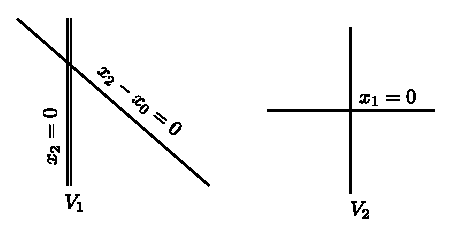
\includegraphics{vol74-figures/1-fig.eps}}
      \end{figure}
      \begin{figure}[H]
        \centering{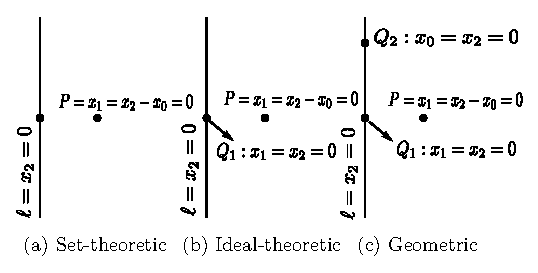
\includegraphics{vol74-figures/2-fig.eps}}
      \end{figure}
  \end{enumerate}
\item ~\pageoriginale
\vskip -1.4cm  
  \begin{align*}
    \rad ((I'_1+I'_2)\bar{R}+\tau\bar{R}) & 
    = (X_2,Y_2,X_0-Y_0,X_1-Y_1)\\
    & \quad \cap (X_2-X_0,X_1,Y_1,X_0-Y_0,X_2-Y_2)\\
    & = \mathscr{Y}_{1,2} \cap \mathscr{Y}_{1,1}
  \end{align*}
  $$
  \displaylines{\text{where}\hfill \mathscr{Y}_{1,2} \coloneqq
    (X_2,Y_2,X_0-Y_0,X_1-Y_1)\hfill \cr 
    \text{and}\hfill \mathscr{Y}_{1,1}=
    (X_2-X_0,X_1,Y_1,X_0-Y_0,X_2-_2).\hfill } 
  $$
  \begin{align*}
    \delta & = \dim (V_1) + \dim (V_2) + 2 = 1 + 1 + 2 = 4\\
    d & = \dim (V_1 \cap V_2) + 1 = 1 + 1 = 2\\
    t & = 1.  \text{ Therefore }  \delta - d -1 = 1.
  \end{align*}
  Following the proof of Step \ref{chap2:sec3:step1} in Chapter II, we get:
\item ~
\vskip -1.4cm
  \begin{align*}
    U([(I'_1 + I'_2)\bar{R}]_1) &= (I'_1 + I'_2)\bar{R} +
    (\ell_0,\ell_1)\bar{R}\\ 
    & = q_{1,2}\cap \mathscr{O}_1
  \end{align*}
  where $q_{1,2} = (X^2_2,Y_2,\ell_0,\ell_1)$ is the
  $\mathscr{Y}_{1,2}$- primary component of $U([(I'_1+
    I'_2)\bar{R}]_1)$ and  
  $$
  \mathscr{O}_1 = (X_2-X_0,Y_1,\ell_0,\ell_1)\cap
  (X^2_2,Y_1,\ell_0,\ell_1) \cap (X_2-X_0,Y_2,\ell_0,\ell_1).
  $$ 
\item Let $C_1$ be the irreducible component of $V_1 \cap V_2$
  corresponding to the prime ideal $\mathscr{Y}_{1,2}$. Then the
  defining prime ideal\pageoriginale of $C$ is $\mathscr{Y}(C) = (X_2) \subset$
  $K[X_0, X_1, X_2]$ and 
  $$
  j(V_1,V_2;C) = ~\text{length of}~ q_{1,2} = \ell
  ((\overline{R}/q_{1,2})_{\mathscr{Y}1,2}) = 2
  $$
  Note that $t < d;$ therefore $\mathscr{O}_1 \neq \bar{R}$.
  
  Now following the proof of step \ref{chap2:sec4:step2} in Chapter
  II, we get:  
  
\item $U(\mathscr{O}_1, \ell_2)=q_{1,1} \cap q_2 \cap q'_2$ where 
  $q_{1,1} = (X_2 -X_0, Y_1, \ell_0, \ell_1,\ell_3)$ is the
  $\mathscr{Y}_{1,1}$-primary component of $U (\mathscr{O}_1,
  \ell_2)$ and $q_2 =(X{^2_2},Y_1, \ell_0, \ell_1, \ell_2)$ (\resp 
  $q'_2=(X_2-X_0,Y_2,\ell_0, \ell_1, \ell_2)$ is
  $\mathscr{Y}_2=(X_1, Y_1, X_2, Y_2, X_0-Y_0)$ (\resp  
  $ \mathscr{Y}'_{2} = (X_0, Y_0, X_2,Y_2,X_1,-Y_1))$ -primary
  component of $U (\mathscr{O}_1,\ell_2)$ 
\item Let $C_2$ be the irreducible component of $V_1 \cap V_2$
  corresponding to the prime ideal $\mathscr{O}_{1,1}$ and let
  $C_3, C_4$ be irreducible subvarieties of $V_1 \cap V_2$
  corresponding to the prime ideals $\mathscr{Y}_2,\mathscr{Y}'_2$,
  respectively. Then the defining prime ideals of $C_2, C_3$ and
  $C_4$ are $(X_2 -X_0, X_1)$, $(X_1, X_2^2)$ and $(X_2 -X_0,X_2)$
  respectively and 
  \begin{align*}
    j(V_1,V_2;C_2)& = \text{length of}~ q_{1,1} = 1\\
    j(V_1,V_2;C_3) &= \text{lent of}~ q_2 = 2\\
    j(V_1,V_2;C_4) &= \text{Lent of}~ q'_3 = 1
  \end{align*} 
  
  Note that $\mathscr{O}_{d-t+1} = \mathscr{O}_2 = \bar{R}$ and
  therefore there is no step \ref{chap2:sec5:step3} in this example 
\item (a) The required collection $\{ C_i\}$ of irreducible
  subvarieties of $V_1 \cap V_2$ is:   
  \begin{align*}
    C_1:  X_2 & = 0 \text{ the line } \ell \text{ with } j (V_1, V_2
    ;C_1) = 2.\\ 
    C_2:  X_1 & =X_2-X_0 = 0 \text{(the isolated point P) with } j
    (V_1, V_2 ;C_2) = 1.\\ 
    C_3:  X_1 & = X_2 = 0\text{(the imbedded point }Q_1) \text{
      with} j (V_1, V_2 ;C_3) = 2.\\ 
    C_4:  X_0 & = X_2 =0  \text{(the geometric imbedded point} Q_2)
    \text{with}\\ 
    & \qquad \qquad j (V_1, V_2 ;C_4) = 1.
  \end{align*}\pageoriginale  
  (b) From \ref{chap1:sec3:subsec1.35}, we have $\deg (V_1) = 3, \deg
  (V_2) = 2$ and $\deg 
  (C_i) = 1$ for all $i = 1,\ldots,4$.  therefore we get  
  $$
  6 = \deg (V_1).\deg (V_2) = \sum_{i=1}^4 j (V_1, V_2 ;C_i) \deg (C_i) = 6.
  $$
\end{enumerate}
\end{example}

\setcounter{example}{2}
 \begin{example}\label{chap3:sec1:exp3.3}%The(3.3)
  Let $V$ be the non-singular curve in $\mathbb{P}^3_K,$
  parametrically given by $\{ s^4, s^3t, st^3,t^4\}$ ( see
  [\cite{26}, p.180], [\cite{50}, p.126]; [\cite{90}, \S 11] and (0.5)) 
\end{example}

It is easy to see that the prime ideal of $V$ is 
\begin{multline*}
I=(X_0 X_3-X_1 X_2,X^2_0 X_2 - X_1^3, X_1 X^2_3 -X^2_3, X_0 X^2_2 -
X^2_1  X_3)\\ 
\subset K[X_0,X_1,X_2,X_3]. 
\end{multline*}
Let $V_1 \subset \mathbb{P}^3_K$ be the defined by $X_0 = X_1 =
0$. Then $I_1 = (X_0,X_1) \subset K[X_0, X_1, X_2, X_3]$ is the prime
ideal of $V_1$. It is  easy to see that: 
\begin{enumerate}[(i)]
\item $(I+I_1) = (X_0, X_1,X^3_2)$ is $\mathscr{Y} = (X_0, X_1, X_2,
  )$ -primary; therefore the intersection $V \cap V_1$ has precisely
  one isolated point $p:  X_0 = X_1 =  X_2 = 0 $. 
\item $\rad ((I'+I'_1) \bar{R} + \tau \bar{R}) = \mathscr{Y}_{1,1}$, where

  $\mathscr{Y}_{1,1} = (X_0, X_1, X_2, Y_0, Y_1, Y_2, X_3 - Y_3)$

  $\delta = \dim V+ \dim V_1 + 2 = 1 + 1 + 2 = 4 $

  $d =\dim (V \cap V_1)+1 = 1, t=1$.\pageoriginale Therefore $t=d$ and $\delta-d-1
  =2$. Following the proof of Step \ref{chap2:sec3:step1} in Chapter
  II, we get:   
\item $U([I' + I'_1) \bar{R}]_2 = q_{1,1} \cap \mathscr{O}_1$ where
  $q_{1,1}$ is $\mathscr{Y}_{1,1}$ primary component of $U([I' + I'_1)
  \bar{R}]_2)$ and $((I' + I') \bar{R} + (\ell_0,\ell_1,\ell_2)
  \bar{R})_{\mathscr{Y}_{1,1}}= U([I' + I'_1)
    \bar{R}]_2)_{\mathscr{Y}_{1,1}}$. Therefore
  $(q_{1,1})_{\mathscr{Y}_{1,1}} = (X_0, X_1, X^3_2,
  Y_0,Y_1, X_2-Y_2, X_3-Y_3) \bar{R}_{\mathscr{Y}_{1,1}}$  
\item Let $C_1$ be the irreducible component of $V \cap V_1$
  corresponding to the prime ideal $ \mathscr{Y}_{1,1}$. Then the
  defining prime ideal of $C_1$ is $(X_0, X_1, X_2) = \mathscr{Y}$ and  
  $$
  j(V, V_1 ; C_1) \text{ length } (q_{1,1})=3
  $$

Note that $t = d =1$ therefore their is no Step \ref{chap2:sec4:step2} in this
example. Following  Step \ref{chap2:sec5:step3} in Chapter II, we get $K -\dim
U(\mathscr{O}_1, \ell_3) = K \dim  (\mathscr{O}_1, \ell_3) = K -\dim
(\mathscr{O}_1) -1 = 0$ Therefore $q:  = U (\mathscr{O}_1, \ell_3) =
(\mathscr{O}_1, \ell_3)$ is primary ideal corresponding to the
homogeneous maximal ideal $(X_0, Y_0, X_1, Y_1,X_2,Y_2,X_3$, $Y_3)
\subset \bar{R}$  This primary ideal $q$ gives the empty subvariety
$\phi$ in our collection.  
\item 
  \begin{enumerate}[(a)] 
    \item The required collection $\{C_i\}$ of irreducible
      subvarieties  of $V \cap V_1$ is:  

      $C_1:  X_0 = X_1 = X_2 =0$ (the isolated point $P$) with $j(V,
      V_1,C_1)\break = 3$, $\phi$: the empty subvariety with $ j(V, V_1 ; \phi )
      $ = length of $(q)$ 

    \item From\pageoriginale (\ref{chap1:sec3:exp1.43}) (iii) and
      \ref{chap1:sec3:subsec1.35}), we have $\deg
      (V) = 4$ and $\deg (V_1)\break = 1, \deg (C_1) = 1$. 
    \item Therefor, from the main theorem  \ref{chap2:sec1:subsec2.1} we get 
  \begin{align*}
    4 =\deg (V). \deg (V_1) &= j (V, V_1 ; C_1) \deg C_1 + j (V, V_1,
    \phi). \deg (\phi)\\ 
    &= 3 + j (V, V_1, \phi).
  \end{align*}
  \end{enumerate}
  This shows that $j(V, V_1, \phi)$ = length of $(q) = 1$, so that $q
  =( \mathscr{O}_1, \ell_3)$ is the homogeneous maximal ideal $(X_0,
  X_1, X_2, X_3, Y_0, Y_1 Y_2, Y_3)$. 
\end{enumerate}

The line $V_1$ is a tangent line to $V$ at $P$ whose intersection
multiplicity with $V$ at $P$ is $3$. In general, the non-singular
curves $C_d \subset \mathbb{P}^3_K$ defined parametrically by 
$$
\left\{ s^d, s^{d-1}t, st^{d-1}, t^d\right\}, d \geq 4, 
$$
are of degree $d$ and have a tangent line with a contact of order
$d-1$ 

\setcounter{remark}{3}
\begin{remark}\label{chap3:sec1:rem3.4}
  The empty subvariety $\phi$ is geometric imbedded component of $V \cap
  V_1$ in example (\ref{chap3:sec1:exp3.3}). 
\end{remark}

\setcounter{example}{4}
\begin{example} \label{chap3:sec1:exp3.5}% exmp (3.5)
  Let $V \subset \mathbb{P}^3_K$ be the non-singular curve of example
  (\ref{chap3:sec1:exp3.3}) and $ V_2 \subset \mathbb{P}^3_K $ be the line defined by $X_0 =
  X_2 = 0$. Then  $I_2 = (X_0, X_2) \subset K [X_0,X_1,X_2,X_3]$ be the
prime ideal of $V_2$. It is easy to see that: 

\begin{enumerate}[(i)] 
  \item The primary decomposition of $I + I_2$ is given by $I + I_2 =
    (X_0, X_1, X_2)\break \cap (X_0,X_1, X^3_1,X^2_3,X^2_1 X_3)$  and
    therefore $\rad (I+I_2) = (X_0,X_1,X_2)$.\pageoriginale 
  \item The set-theoretic intersection $V \cap V_2$ of $V$ and $V_2$
    has precisely one isolated point. 
  \item $\rad (( I' +I'_2) \bar{R} + \tau \bar{R}) = \mathscr{Y}_{1,1}$ where 

    $\mathscr{Y}_{1,1} = (X_0,X_1,X_2, Y_0,Y_1,Y_2,X_3-Y_3)$.

    $\delta = \dim V +\dim V_2 + 2 = 1+ 1 + 2 = 4$

    $ d = \dim (V \cap V_2) + 1 = 1, t = 1$. Therefore $ t = d$ and
    $\delta -d-1 =2$.  

    Following the proof of step \ref{chap2:sec3:step1} is Chapter II, we get:
    $$
    U([(I' + I'_2) \bar{R}]_2) = q_{1,1} \cap \mathscr{O}_1
    $$
    where $q_{1,1}$ is $\mathscr{Y}_{1,1}$ -primary component of
    $U([(I' + I'_2) \bar{R}]_2)$ and 
    \begin{align*}
      (q_{1,1}){_\mathscr{Y}}{_{1,1}} U([(I' + I'_2)
        \bar{R}]_2)_{\mathscr{Y}_{1,1}} &= (I' + I'_2)
      \bar{R}+(\ell_0, \ell_1,\ell_2) \bar{R}_{\mathscr{Y}_{1,1}} \\ 
      & = (X_0,X_1,X_2, Y_0,Y_1,Y_2,X_3-Y_3).
    \end{align*}
 \item Let $C_1$ be the irreducible component of $V_1 \cap V_2$
   corresponding to the prime ideal $\mathscr{Y}_{1,1}$. Then the
   defining prime ideal of $C_1$ is $(X_0,X_1, X_2 ) = \mathscr{Y}$ and
   $j(V, V_2 ;C_1)=$ length of $q_{1,1} = 1$ Note that $t = d = 1 ;$
   therefore there is no Step \ref{chap2:sec4:step2} in this
   example. Following Step \ref{chap2:sec5:step3} in Chapter II, we get 
   
   $K - \dim (\mathscr{O}_1, \ell_3) = K -\dim U(\mathscr{O}_1, \ell_3)=
   K- \dim (\mathscr{O}_1)-1 = 0$.  

   Therefore $q:  = U(\mathscr{O}_1, \ell_3) = (\mathscr{O}_1, \ell_3)
   $ is primary ideal corresponding to the homogeneous maximal ideal
   $(X_0,X_1,X_2,X_3, Y_0,Y_1,Y_2$, $Y_3) \subset \bar{R}$. This primary
   ideal $q$ gives empty subvariety $\phi$ in our collection  

  \item (a)\pageoriginale The required collection $\{C_i\}$ of irreducible
    subvarieties of $V \cap V_2$ is:  

    $C_1:  X_0 = X_1 = X_2 = 0$ (the isolated point $P$) with $j (V,
    V_2 ; C_1) =1$. $\phi$: the empty subvariety with $j (V, V_2 ;
    \phi) =$ length of $q$ 

    (b) We have from example(\ref{chap3:sec1:exp3.3}) $\deg (V) = 4$
    and from \ref{chap1:sec3:subsec1.35} 
    $$
    \deg (V_2) = 1, \deg (C_1) = 1 
    $$
    
    (c) Therefore from the main theorem we get  
    \begin{align*}
      4 = \deg (V). \deg (V_2) &= j(V, V_1,V_2 ;C_1) \deg (C_1)\\ 
      & \qquad + j(V, V_1, V_2 ; \phi) \deg (\phi)\\ 
      &=1+j (V, V_1, V_2 ; \phi)
    \end{align*}
\end{enumerate}
\end{example}

    This shows that $j (V, V_1, V_2 ; \phi)$ = length of $q = 3$.

\setcounter{remark}{5}
\begin{remark}\label{chap3:sec1:rem3.6}
  The empty subvariety $\phi$ is imbedded component of $V \cap V_2$ in
  example (\ref{chap3:sec1:exp3.5}) 
\end{remark}

\setcounter{example}{6}
\begin{example}\label{chap3:sec1:exp3.7}
  Let $V_1$ and $V_2$ be two hypersurfaces in $\mathbb{P}^2_K$ defined
  by $F_1:  = X_0 X_1 (X_0 -2X_1) = 0$ and $F_2:  = X_0 X_1 (X_1 -2X_0)
  = 0$. put $I_1  = (F_1)$ and $I_2 = (F_2)(\subset K
  [X_0,X_1,X_2])$. It is easy to see that: 
  \begin{enumerate}[(i)]
  \item The primary decomposition of $I_1 + I_2$ is given by $I_1 + I_2
    = (X_0) \cap (X_1) \cap (X^2_0, X^2_1)$ and therefore $\rad (I_1 +
    I_2) = (x_0) \cap (X_1)$.  
  \item (a) The set-theoretic intersection $V_1 \cap V_2$ of $V_1$ and
    $V_2$ is precisely the two lines $\ell_0:  X_0 = 0$ and $\ell_1:
    X_1 = 0$. 
    
    (b)\pageoriginale The ideal-theoretic intersection of $V_1$ and
    $V_2$ is precisely 
    the two lines $\ell_0:  X_0 = 0 \ell_1:  X_1 = 0$ and the imbedded
    point $P:  X_0 = X_1 = 0$ 
  \item $\rad ((I'_1 + I'_2) \bar{R} + \tau \bar{R}) = \mathscr{Y}_{1,2}
    \cap \mathscr{Y}_{2,2} \cap \mathscr{Y}_{1,1} $ where  
    
    $\mathscr{Y}_{1,2} = (X_0, Y_0, X_1 -Y_1, X_2
    -Y_2),\mathscr{Y}_{2,2} = (X_1, Y_1, X_0 -Y_0, X_2 -Y_2) $ and 
    
    $\mathscr{Y}_{1,1} = (X_0, X_1, Y_0 -Y_1, X_2 -Y_2)$.
    
    $\delta= \dim V_1+\dim V_2+2=1+1+2=4$
    
    $d = \dim (V_1 \cap V_2) + 1 = 2, t = 1$ therefore  $\delta-d-1 = 1$ 
    
    Following the proof of Step \ref{chap2:sec3:step1} in Chapter II, we get:
    
    (iv) $\cup ([(I'_1 + I'_2) \bar{R}]_1) = q_{1,2} \cap q_{2,2} \cap
    \mathscr{O}_1$, where $q_{1,2} (\text{\resp } q_{2,2})$ is
    $\mathscr{Y}_{1,2}$ -$(\mathscr{Y}_{2,2})$- primary component of$ U
    ([(I'_1 + I'_2) \bar{R}]_1)$ In fact, $q_{1,2} =(X_0,
    Y_0,\ell_0,\ell_1), q_{2,2} =(X_1, Y_1,\ell_0,\ell_1) $ 
  \item Let $C_1 $ and $C_2$ be irreducible components of $V_1 \cap V_2$
    corresponding to the prime ideals $\mathscr{Y}_{1,2}$ and
    $\mathscr{Y}_{2,2}$. Then the defining prime ideals of $C_1$ and
    $C_2$ are $(X_0)$ and $(X_1)$,respectively and $j(V_1, V_2 ;C_1)= $
    length of  $q_{1,2} = 1,j(V_1, V_2 ;C_2) =$ length of $q_{2,2} =
    1,$, 
    
    Note that $t < d$: therefore $\mathscr{O} _1 \neq \bar{R}$.
    
    Following the proof of step \ref{chap2:sec4:step2} is Chapter II we get: 
  \item $q:  = U (\mathscr{O}_1, \ell_2) = (\mathscr{O}_1, \ell_2)$ is
    $\mathscr{Y}_{1,1}$ - primary ideal. Let $C_3$ be the irreducible
    component of $V_1 \cap V_2$ corresponding to the prime ideal
    $\mathscr{Y}_{1,1}$. Then the defining prime ideal of $C_3$ is $(X_0,
    X_1) $ and $ j(V_1,V_2 ;C_3)$ = length of $(q)$.
    
  \item (a)\pageoriginale The required collection $\{C_i\}$ is: 
    \begin{align*}
      C_1 : X_0 & = 0 ~\text{(the line} ~\ell_0) ~\text{with} ~j(V_1,
      V_2 ; C_1) = 1\\ 
      C_2 : X_1 &= 0 ~\text{(the line} ~\ell_1) ~\text{with} ~j(V_1,
      V_2 ; C_2) = 1\\ 
      C_3 : X_0 &=X_1 = 0 \text{(the imbedded point P ) with} ~j(V_1,
      V_2 ; C_3) =\ell (q) 
    \end{align*}
    
    (b)\pageoriginale From \ref{chap1:sec3:subsec1.35}, we have $\deg
    (V_1) = \deg (V_2) = 3$ and $\deg C_i = 1$ for all $i =1,2,3$. 
    
    (c) from the main theorem \ref{chap2:sec1:subsec2.1}, we get $9 = \deg (V_1) \cdot \deg (V_2) =
  \sum \limits_{i = 1}^3 j (V_1,V_2;C_i) \deg (C_i) = 2+ j
  (V_1,V_2;C_3)$.  
  \end{enumerate}
\end{example}

Therefore $\ell(q) = j (V_1,V_2;C_3) = 7$ 

This example was also studied by $W$. Fulton and $R$. MacPherson in
[\cite{19}, p.10] 

\setcounter{example}{7}
\begin{example}\label{chap3:sec1:exp3.8}
  Let $V_1 = V(I_1)$ and $V_2 = V(I_2) $ be two projective varieties
  in $\mathbb{P}^n_K$ defined by homogeneous ideals $I_1 = (X_4,
  X^3_3-X_1X_2(X_2-2X_1))$ and $I_2 = (X_3, X^3_4-X_1X_2(X_1-2X_2))
  \subset K[X_0,X_1,X_2,X_3,X_4]$. Following the proof of the main
  theorem \ref{chap2:sec1:subsec2.1} it is easy to see that:   
  
  (a)The required collection $\{ C_i\}$ is given by:.
{\fontsize{10pt}{12pt}\selectfont
  \begin{align*}
    C_1:X_1&=X_3=X_4 = 0 ~\text{(the line) with } j(V_1, V_2 ;C_1) = 1\\
    C_2:X_1&=X_3=X_4 = 0 ~\text{(the line) with } j(V_1, V_2 ;C_2) = 1\\
    C_3:X_1&=X_2=X_3=X_4 = 0 ~\text{(the imbedded point) with }
    j(V_1, V_2 ;C_3) = 7. 
  \end{align*}}\relax

  (b) From \ref{chap1:sec3:subsec1.35} we have $\deg (V_1) = \deg
  (V_2) = 3$ and $\deg (C_i) = 1 \text{for}~ i = 1,2,3$. Therefore 
  $$
  9 = \deg (V_1) \deg (V_2) = \sum_{i=1}^3 j(V_1,V_2 ;C_i) \deg (C_i).
  $$
\end{example}

\setcounter{remark}{8}
\begin{remark}\label{chap3:sec1:rem3.9}
  The example (\ref{chap3:sec1:exp3.8}) was also studied by $W$. Fulton and $R$. MacPherson,
  (see [\cite{19},p.10]) This example illuminates our problem 6 below as
  follows: 
  
  Use the diagram for $X: = V_1$ and $Y: =V_2$
    \[
    \xymatrix{X \cap Y \ar[r]\ar[d]& \Delta \ar[d]\\
      X \times Y \ar[r] & \mathbb{P}^4 \times \mathbb{P}^4      
      }
    \]
  the origin $P$ is a so-called distinguished variety in the theory of
  Fulton and MacPherson, its contribution to the multiplicity is $3$,
  each line also contributes $3$ to the Bezout's number $\deg
  (X). \deg (Y) = 9 $. 
  
  In view of the problem $6$ below, we want to consider another
  diagram. Using the diagram 
  \[
  \xymatrix{X \cap Y \ar[r] \ar[d] & X \times Y \ar[d]\\
    \Delta_{\mathbb{P}^4} \ar[r] & \mathbb{P}^4 \times \mathbb{P}^4
    }
  \]  
  then we get the intersection numbers 7,1,1  (7 at the point $P$) by
  applying the theory of Fulton and MacPherson. Our method also\pageoriginale
  assigns the multiplicity $7$ to the origin $P$ and $1$ to each
  line. 
  
  A simpler example in $\mathbb{P}^2_K$ is the following: Let $X$ and
  $Y$ be given by $X_1 X_2 = 0$ and $X_1 = 0$,\resp  Then $X \cap Y$ is
  the line $X_1 = 0$. Applying again the theory of Fulton and
  MacPherson, we will construct intersection from the diagram   
  \[
  \xymatrix{X \cap Y \ar[r]\ar[d] & Y\ar[d]\\
    X \ar[r] & \mathbb{P}_K^2
    }
  \]
  Then only $Y$ is a distinguished variety and counts twice. Construct
  intersection from the diagram 
  \[
  \xymatrix{X \cap Y \ar[r]\ar[d] & X \times Y \ar[d]\\
    \Delta_{\mathbb{P}^2}\ar[r] & \mathbb{P}^2 \times \mathbb{P}^2
    }
  \]
  Then $Y$ and the origin are distinguished varieties each contributes
  $1$. In our theory, the origin is also a so-called distinguished
  variety and its contribution to the multiplicity is $1$, the line
  $X_1 = 0$ also contributes $1$ to the Bezout's number $\deg (X) \deg
  (Y) = 2$. 
\end{remark}

Therefore we want to study the following example:
\setcounter{example}{9}
\begin{example}\label{chap3:sec1:exp3.10}
  Let $V_1$ and $V_2$ be two hypersurfaces in $\mathbb{P}^2_K$
  defined\pageoriginale by $F_1: = X_1X_2 $ and $ F_2: = X^n_1 = 0$ 

  Following the proof of the main theorem \ref{chap2:sec1:subsec2.1},
  it is easy to see that: 

\begin{enumerate}[(a)]
\item The required collection $\{ C_i\}$ is: 

  $\begin{aligned}
  C_1:  X_1 &=0 \text{(the line) with } j (V_1, V_2;C_1) = n\\
  C_2:  X_1 &= X_2 = 0 \text{(the imbedded points) with } j (V_1,
  V_2;C_2) = n 
\end{aligned}$
\item From (\ref{chap1:sec3:subsec1.35}), we have $\deg (V_1) = 2$, $\deg (V_2) = n$ and
 $\deg (C_i)= 1$ for $i = 1,2$. 
  
Therefore $2 n = \deg (V_1). \deg (V_2) =\sum\limits_{i=1}^2 j(V_1,
  V_2 ;C_i) \deg (C_i)$ 
\end{enumerate}
\end{example}

\setcounter{example}{10}
\begin{example}\label{chap3:sec1:exp3.11}
  Let $V_1 = V (I_1)$ and $V_2 = V (I_2)$ be two subvarieties in
  $\mathbb{P}^n_K $ with $ V_1 \cap V_2 = \phi $ (for example,the
  lines $\ell_0:  X_0 = X_1 =0$ and $\ell_1:  X_2 = X_3 =0 $ in $~
  \mathbb{P}^3_K$). Following the proof of the main theorem
  \ref{chap2:sec1:subsec2.1}, it
  is easy to see that:  $d=0,\delta - d- 1 = \delta - 1 \le n $  and $
  U([I'_1 + I'_2]_{\delta-1})=q$ is primary for the homogeneous
  maximal ideal $(X_0,\ldots,X_n, Y_0,\ldots,Y_n)$. Therefore  the
  required collection $\{ C_i\}$ is just the empty subvariety $\phi$
  and by the main Theorem \ref{chap2:sec1:subsec2.1}), we get  
  $$
  j(V_1, V_2 ; \phi)= \deg (V_1)\cdot \deg (V_2).
  $$
\end{example}

\setcounter{remark}{11}
\begin{remark}\label{chap3:sec1:rem3.12}
  Let $V_1 and V_2$ be as in example (\ref{chap3:sec1:exp3.11}). Let
  $C(V_1)$ (\resp   \break $C(V_2)$)
  be the projective cone over $V_1$ (\resp  over $V_2$) in
  $\mathbb{P}^{n+1}_k$. Then $C(V_1) \cap C(V_2)$ is given by one point
  say $P:X_0=\dots=X_n = 0$. It is possible to show that   
  $$
  j(V_1, V_2 ; \phi)= j(C(V_1), C(V_2); P).
  $$
  which\pageoriginale does provided a geometrical interpretation of the intersection
  number $ j (V_1, V_2 ;\phi)$. 
\end{remark}

\setcounter{subsection}{12}
\subsection{} \label{chap3:sec1:subsec3.13}
Let $V_1, V_2$ and $V_3 \subset \mathbb{P}^3_K$ be three
hypersurfaces defined by $F_1: = X_0X_1,\break F_2:  X_0 X_2$ and  $F_3:
X_0X_3$, respectively. Put $I_1 = (F_1), I_2 = (F_2)$ and $I_3 =
(F_3) (\subset K[X_0, X_1,X_2,X_3])$. It is easy to see that: 

\begin{enumerate}[(i)] 
\item 
  The primary decomposition of $I_1 + I_2 + I_3$ is given by $I_1 +
  I_2 + I_3 = (X_0) \cap (X_1,X_2,X_3)$ and $\rad (I_1 + I_2 + I_3) = (X_0)
  \cap (X_1,X_2,X_3)$. Therefore the intersection $V_1 \cap V_2 \cap
  V_3$ is precisely one surface $C: X_0 = 0$  and the isolated point
  $P:  X_1 = X_2 = X_3 = 0$. 

  Note that we cannot apply the main theorem
  \ref{chap2:sec1:subsec2.1} to this example but 
  we can apply the general main theorem
  \ref{chap2:sec5:subsec2.25}. We preserve the 
  notation of \cite{56}. For simplicity, put $X_{ij} = X_j, X_{2j} = Y_j
  \text{and} X_{3j} = Z_j$ for $j = 0,\ldots,3$.   
\item  $\rad ((I'_1 + I'_2 +I'_3) \bar{R} +\tau \bar{R}) =\mathscr{Y}_{1,3}
  \cap \mathscr{Y}_{1,1}$ where $\mathscr{Y}_{1,3} = (X_0, Y_0,Z_0,X_1-Y_1,X_1
  -Z_1,X_2-Z_2,X_3-Y_3,X_3,-Z_3)$ and   

  $\mathscr{Y}_{1,1} = (X_1,
  Y_1,Z_1,X_2,Y_2,Z_2,X_3,Y_3,Z_3,X_0,-Y_0,X_0,-Z_0)$ and 
 
  $\delta =\dim V_1 + \dim V_2 + \dim V_3 + 3 =2 + 2 +2 +3 = 9$,
   
  $\delta= \dim (V_1 \cap V_2 \cap V_3)+1 = 3, t=1$. Therefore
  $\delta-d-1 =9 -3-1=5$  
    
  Following the proof of Step \ref{chap2:sec3:step1} of [\cite{56},
    \ref{chap2:sec1:subsec2.1}], we get:
\item $U([(I'_1 + I'_2 + I'_3) \bar{R}]_5) = q_{1,3} \cap
    \mathscr{O}_1$ where $ q_{1,3} = (X_0,
    Y_0,Z_0,\ell_0,\ldots,\ell_5)$ is the $\mathscr{O}_{1,3}$ primary
    component of $U([(I'_1 + I'_2 + I'_3) \bar{R}]_5)$ 
\item Let\pageoriginale $C_1$ be the irreducible component of $V_1 \cap V_2 \cap V_3$
    corresponding to the prime ideal $\mathscr{O}_{1,3}$. Then the
    defining prime ideal of $C_1$ is $(X_0)$ and  $j (V_1, V_2,V_3 ;
    c_1)$ = length of $q_{1,3} = 1$. Following the proof of Step
    \ref{chap2:sec4:step2} of \cite{56}, \ref{chap2:sec1:subsec2.1}, we get: 
\item $\cup(\mathscr{O}_1, \ell_6)=  q_1^1 \cap q_1^2 \cap q_1^3 \cap
  \mathscr{O}_2$ where $q_1^1$ (\resp  $q_1^2,q_1^3$) is
  $(X_1,Y_0,Z_0)+ \tau \bar{R}$ (\resp  $(X_0,Y_2,Y_0)+ \tau \bar{R}
  (X_0, Y_0, Z_3)+ \tau \bar{R}$)-primary components of $U
  (\mathscr{O}_1, \ell_6)$. Let $C_2, C_3 
  \text{and} C_4$ be irreducible subvarieties of $V_1 \cap V_2 \cap V_3$
  corresponding to the prime ideals $(X_1,Y_0,Z_0)+ \tau\bar{R}
  (X_0,Y_2,Z_0)+ \tau\bar{R}$ and $(X_0,Y_0,Z_3)+ \tau\bar{R}$
  respectively. Then the defining prime  ideals of $C_2, C_3$ and
  $C_4$ are $(X_0, X_1), (X_0,X_2)$ and $(X_0, X_3),$ respectively and
  $j(V_1,V_2,C_i)$ = 1 for $i = 2,3,4$. 

\item  $\cup(\mathscr{O}_2, \ell_7)=  q_1^1 \cap q_1^2 \cap q_1^3 \cap
  q_1^4 $ where 
  
  $q_1^1 = (X_0,Y_2,Z_3)+ \tau \bar{R} q^2_1 = (X_1,Y_0,Z_3)+\tau \bar{R}
  q_1^3 = (X_0,Y_2,Z_0)+\tau \bar{R}$ and 

  $q_1^4 = (X_0,Y_2,Z_3)+\tau \bar{R}$

  Note that $d-t+1=3$ and $\mathscr{O}_{d-t+1} = \mathscr{O}_3 =
  \bar{R}$. Let $C_5, C_6,C_7$ and $C_8$ be irreducible. subvarieties
  of $V_1 \cap V_2 \cap V_3$ corresponding  to $q_1^1, q^2_1,q^3_1$
  and $q^4_1$, respectively. Then the defining prime ideals of $C_5,
  C_6,C_7$  and $C_8$ are $(X_0,X_2,X_3),
  (X_0,X_1,X_3),(X_0,X_1,X_2)$, and $(X_1,X_2,X_3)$ respectively and
  $j (V_1, V_2,V_3,C_i) = 1$ for  $i= 5,6,7,8$. 
\item (a) The required collection $\{ C_i\}$ is:
  \begin{align*}
    C_1 &: X_0 = 0 \quad \text{(the surface)}\\
    C_2 &: X_0=X_1=0 \\
    C_3 &: X_0 = X_2=0 \\
    C_4 &: X_0 = X_3=0 \\
    C_5 &: X_0 = X_2= X_3 =0\\
    C_6& : X_0 = X_1= X_3 =0 \\
    C_7& : X_0 = X_1= X_2 =0 \\
    C_8& : X_1 = X_2= X_3 =0 \quad \text{(the isolated point)}
  \end{align*}
and\pageoriginale $j(V_1, V_2 ;C_i) = 1$ for all $i = 1,\ldots,8$.

(b) From \ref{chap1:sec3:subsec1.35}, we have

$\deg (V_i) = 2$ for all $i = 1,2,3$ and $\deg (C_i) = 1$ for all $i =
1,\ldots,8$. Therefore we get  $8 =\prod\limits_{i=1}^3 \deg (V_i) =
\sum\limits_{i=1}^8 j(V_1, V_2;C_i) \deg (C_i)$.  
\end{enumerate}

\setcounter{examples}{13}
\begin{examples}\label{chap3:sec1:exp3.14}
\begin{enumerate}[(i)] 
\item Let $V_1 =V(I_1)$ and $V_2 =V(I_2) \subset \mathbb{P}^7_K$ be
  defined  by $I_1 = (X_0,X_1) \cap (X_2,X_3) \cap (X_4,X_5) \cap
  (X_6,X_7) $ and $I_2= (X_0 +X_2,X_4+X_6)$. Then the primary
  decomposition of $I_1 + I_2$ is given by   
{\fontsize{10pt}{12pt}\selectfont
  \begin{multline*}
    I_1+ I_2 =(X_0,X_1,X_2,X_4+X_6) \cap (X_0,X_2,X_3,X_4+X_6)\\ 
    \cap (X_4,X_5,X_6,X_0+X_2) \cap (X_4,X_6,X_7,X_0+X_2)\\ 
    \cap (X_0^2,X_2^2,X_0+X_2,X_1,X_3,X_4+X_6)
    (X_4^2,X_6^2,X_4+X_6,X_5,X_7,X_0,+X_2). 
  \end{multline*}}\relax

  Using the notation of \ref{chap2:sec6:subsec2.30} we have
  $$
  m = 4, \ell =6.
  $$

  We also have $3 =\dim (V_1 \cap V_2) = \dim (V_1) + \dim
  (V_2)-7=5+5-7=3$ and\pageoriginale from \ref{chap1:sec3:subsec1.40}
  and \ref{chap1:sec3:subsec1.35} $\deg (V_{1}) = 4, \deg (V_{2}) = 1$.  
  Therefore $4 = \deg (V_{1}) \deg (V_{2}) \not \ge \ell - 1 = 5$. 
  This example shows that Question \ref{chap2:sec6:qus1} of
  \ref{chap2:sec6:subsec2.30} is not true in general.  
\item Let $V_{1} = V(I_{1})$ and $V_{2} = V(I_{2}) \subset
  \mathbb{P}^{4}_{K}$ be defined by $I_{1} = (X_{0}, X_{1}) \cap
  (X_{2}, X_{3}) \cap (X_{0} + X_{2}, X_{4})$ and $I_{2} = (X_{0}+
  X_{2})$. Then the primary decomposition of $I_{1} + I_{2}$ is given
  by  
  \begin{multline*}
  I_{1} + I_{2} = (X_{0} + X_{2}, X_{4}) \cap (X_{0}, X_{1}, X_{2})
  \cap (X_{0}, X_{2}, X_{3})\\ 
  \cap (X^{2}_{0},X^{2}_{2}, X_{0} + X_{2}, X_{1}, X_{3} ). 
  \end{multline*}

  Therefore $m = 1$ and $\ell = 4$

  Also $2 = \dim (V_{1} \cap V_{2}) > \dim V_1+ \dim V_{2} -4 = 2 + 3 -4 = 1$
  and $\deg (V_{1}) = 3, \deg (V_{2}) = 1$ by \ref{chap1:sec3:subsec1.39} and
  (\ref{chap1:sec3:rem1.34}). Therefore $3 = \deg (V_{1}) \deg (V_{2})
  \not \ge \ell = 4$. 
  
  This example shows that Question \ref{chap2:sec6:qus2} of
  \ref{chap2:sec6:subsec2.30} is not true in general. 
\item Let $V_{1} = V (I_{1})$ and $V_{2} = V(I_{2}) \subset
  \mathbb{P}^{7}_{K}$ be defined by $I_{1} = (X^{2}_{0}, X_{1}) \cap
  (X_{2}, X_{3}) \cap (X_{4}, X_{5}) \cap (X_{6}, X_{7})$ and $i_{2} =
  (X_{0} + X_{2}, X_{4} + X_{6})$. The primary decomposition of $I_{1}+
  I_{2}$ is given by  
{\fontsize{10pt}{12pt}\selectfont
  \begin{multline*}
    I_{1}+I_{2} = (X^{2}_{0}, X_{1}, X_{0} + X_{2}, X_{4} + X_{6})
    \cap (X_{0}, X_{2}, X_{3}, X_{4} + X_{6})\\ 
    \cap (X_{4}, X_{5}, X_{6}, X_{0} + X_{2})  
    \cap (X_{4}, X_{6}, X_{7}, X_{0} + X_{2}) \cap \\
    (X^{3}_{0}, X^{3}_{0}, X_{1}, X_{3}, X_{0}+ X_{2}, X_{4}, + X_{6})
    \cap (X^{3}_{4}, X^{2}_{6}, X_{5}, X_{7}, X_{0} +  X_{2}, X_{4} + X_{6})
  \end{multline*}}\relax
\end{enumerate}
\end{examples}

  Therefore $m = 4$ and $\ell = 6$. From \ref{chap1:sec3:subsec1.40}
  and \ref{chap1:sec3:subsec1.35} we have $\deg 
  (V_{1}) = 5, \deg (V_{2}) = 1$. Therefore $\deg (V_{1})\cdot \deg (V_{2})
  > m$ but \break $\deg (V_{1})\cdot \deg (V_{2}) \not \ge \ell$. This example
  shows that Question \ref{chap2:sec6:qus3} of
  \ref{chap2:sec6:subsec2.30} is not true in general.   

\section{Applications of the Main Theorem}\label{chap3:sec2}

The\pageoriginale purpose of this section is to show that the main
theorem \ref{chap2:sec1:subsec2.1} also yields Bezout's Theorem. 

We preserve the notation of Chapter II. In addition, the
  following notation will be used in sequel. 

\setcounter{notation}{14}
\begin{notation}\label{chap3:sec2:not3.15}
  Let $V_{1} = V(I_{1})$ and $V_{2} = V(I_{2})$ be two pure
  dimensional projective varieties in $\mathbb{P}^{n}_{K}$ defined by
  homogeneous ideals $I_{1}$ and $I_{2}$ in $R_{0}:  = K [X_{0},
    \ldots,  X_{n}]$. Let $C$ be an irreducible component of $V_{1}
  \cap V_{2}$ with the defining prime ideal $\mathscr{Y}(C) =
  \mathscr{Y}$. Let $q(C) = q$ be the primary component of $I_{1} +
  I_{2}$. we put:  
  \begin{align*}
    \ell (V_{1}, V_{2} ; C) &:  =  ~\text{length of}~ q = \ell
    ((R_{0}/ I_{1} + I_{2}) \mathscr{Y}) ~\text{and} \\ 
    e(V_{1}, V_{2}; C) &: = e_{0} (q(R_{0})_{\mathscr{Y}} ; (R_{0})_{\mathscr{Y}}).
  \end{align*}
\end{notation}

Using (\ref{chap2:sec2:lem2.3}) (iii), we get the isolated prime ideal
$P (\text{\resp}~ 
\bar{P}$) of $(I'_{1} + I'_{2} + \tau)\, R \,(\text{\resp}~ (I'_{1} + I'_{2} +
\tau)\bar{R} )-$ Let $Q \,(\text{\resp}~ \bar{Q})$ be the
$P\,(\text{\resp}~ \bar{P}) - $ 
primary component of $(I'_{1} + I'_{2} + \tau)$  $R \,(\text{\resp}~ (I'_{1} +
I'_{2} + \tau)\bar{R})$. Let $A = (R/(I'_{1} + I'_{2}))_{P} \,(\text{\resp}~
\bar{A} = (\bar{R}/(I'_{1} + I'_{2}))_{\bar{P}}$ be the local ring of
the join-variety $J(V_{1}, V_{2})$ $(\text{\resp}~ \bar{J}(V_{1}, V_{2}))$ at $P
\,(\text{\resp}~ \bar{P})$.

\setcounter{remarks}{15}
\begin{remarks}\label{chap3:sec2:rem3.16}
  \begin{enumerate}[(i)] 
  \item Note that $\bar{P} = \mathscr{Y}_{i, j}$ for some prime ideal
    $\mathscr{Y}_{i,j}$ in $(*)$ of (\ref{chap2:sec2:not2.4}), where
    $j = K -\dim (C)$.  
  \item ~
    \vskip -1.5cm  
    \begin{align*}
      e_{0}(\tau A; A) &  = e_{0}(QA;A) \text{ and }\\
      e_{0} (\tau \bar{A};\bar{A}) &  = e_{0}(\bar{Q}\bar{A};A)
    \end{align*}
  \item ~
    \vskip -1.5cm 
    \begin{align*}
      e_{0}(\tau A; A) &  = e_{0}(\tau\bar{A};\bar{A}) \text{ and}\\
      e_{0} (Q A; A) &  = e_{0}(\bar{Q}\cdot \bar{A};\bar{A})
    \end{align*}
  \end{enumerate}
\end{remarks}

\begin{proof}
(ii)\pageoriginale We have $(QA)^{n} = ((I'_{1} + I'_{2} + \tau)A)^{n}
  = (\tau A)^n$ for all $n 
  \ge 1$, so that $\ell (A/(QA)^{n}) = \ell(A/(\tau A)^{n})$ for all
  $n \ge 1$. Therefore $E_{0}(Q A,A) = e_{0}(\tau A, A)$. Similarly,
  $e_{0}(\bar{Q}.\bar{A}; \bar{A}) = e_{0}(\tau \bar{A}; \bar{A})$.    

  (iii) This follows from the remark (i) of \ref{chap1:sec1:subsec1.2}. 
\end{proof}

\setcounter{remark}{16}
\begin{remark}\label{chap3:sec2:rem3.17}
  If $C$ is a proper component of $V_{1} \cap V_{2}$, that is, $C$ is
  irreducible and $\dim (C) = \dim (V_{1}) + \dim (V_{2}) - n$,then the
  ~\textit{Weil's intersection multiplicity symbol} $i (V_{1},
  V_{2};C)$ of $V_{1}$ and $V_{2}$ along $C$ is given by  
  $$
  i (V_{1}, V_{2};C) = e_{0}(\tau A;A)
  $$
\end{remark}

\begin{proof}
  See [\cite{69} ; ch. II, \S 5, a]
\end{proof}

\setcounter{lemma}{17}
\begin{lemma}\label{chap3:sec2:lem3.18}
  Let $V_{1} = V(I_{1})$ and $V_{2} = V(I_{2})$ be two pure dimensional
  projective varieties in $\mathbb{P}^{n}_{K}$ defined by
  homogeneous ideals ~$I_{1}$ and $I_{2}$ in $R_{0}:  = K[X_{0},
    \ldots,  X_{n}]$. Let $C$ be an irreducible
  component of $V_{1} \cap V_{2}$. Then $j(V_{1},
  V_{2} ;C) = e_{0} ((\ell_{0}, \ldots,\ell_{\delta-j-1}) \bar{A};
  \bar{A}) = \ell_{0}, \ldots,  \ell_{\delta-j-1})\bar{A}) - \ell
  (\dfrac{(\ell_{0}, \ldots, \ell_{\delta-j-2}):
  \ell_{\delta-j-1}}{(\ell_{0},
  \ldots,\ell_{\delta-j-2})\bar{A}})$ where $j=K- \dim (C)$. 
\end{lemma}

\begin{proof}
  This follows from (\ref{chap2:sec4:coro2.20}),
  (\ref{chap2:sec2:prop2.8}) and (\ref{chap1:sec2:def1.23}). 
\end{proof}

\setcounter{corollary}{18}
\begin{corollary}\label{chap3:sec2:coro3.19}
\begin{multline*}
  J(V_{1}, V_{2} ;C)= \ell (V_{1}, V_{2};C) + \ell (\tau
  \bar{A}/(\ell_{0}, \ldots,\ell_{\delta-j-1})\bar{A})\\ 
  - \ell (\dfrac{(\ell_{0}, \ldots, \ell_{\delta-j-2}):
    \ell_{\delta-j-1}}{(\ell_{0}, \ldots,\ell_{\delta-j-2})\bar{A}})
\end{multline*} 
\end{corollary}

\begin{proof}
  We\pageoriginale have $ \ell(V_1,V_2;C) = \ell(\bar{A}/ \tau
  \bar{A})$. Therefore 
  this corollary follows from (\ref{chap3:sec2:lem3.18}). 
\end{proof}
We put
$$
\displaylines{\hfill
  K_1: = \ell( \tau \bar{A}/ (\ell_0,  \ldots\ell
  _{\delta - j-1 })A)~\hfill \cr
  \text{and}\hfill  K_2: = \frac{((\ell_0, \ldots, \ell _ {\delta-j-2}):
    \ell_{\delta-j-1}) \bar{A}}{(\ell_0, \ldots, \ell _{\delta-j-2})
    \bar{A}}\hfill}
$$ 

\begin{corollary}\label{chap3:sec2:coro3.20}
  \begin{enumerate}[(i)] 
  \item  Suppose that the local rings  $A(V_i;C)$  of $V_i$
    at $C$ are Cohen-Macaulay for  $i=
    1,2$. Then $j(V_1,V_2; C) \geq \ell (V_1,V_2;C)$ and
    equality holds if  and only if $\tau \bar{A} \subset (\ell_0,\ldots,\ell
    _{\delta-j-1})\bar{A}$ 

  \item If $\tau \bar{A}\subset (\ell_0, \ldots,\ell
    _{\delta-j-1})\bar{A}$  then $j(V_1,V_2;C) \leq  \ell
    (V_1,V_2;C)$ and equality holds if and only if  $A(V_1;C)
    $ and $A(V_2;C)$ are Cohen-Macaulay. (Note that $\tau \bar{A}\subset
    (\ell_0, \ldots,\ell _{\delta -j-1})\bar{A}$ when $\dim C= \dim\break V_1
    + \dim V_2 - n)$. 
  \end{enumerate}
\end{corollary}

\begin{proof}
  \begin{enumerate}[(i)] 
  \item From the proposition (\ref{chap3:sec2:prop3.21}) below, it follows that $\bar{A}$ is
    Cohen -Macaulay. Therefore (i) results from (\ref{chap3:sec2:coro3.19}). 
  \item Follows from (\ref{chap3:sec2:coro3.19}) and the following
    proposition (\ref{chap3:sec2:prop3.21}). 
  \end{enumerate}
  We study the connecting between the Cohen -Macaulay properties of
  $A(V_i; C)$ and $ \bar{A}$ in the following proposition. 
\end{proof}

\setcounter{proposition}{20}
\begin{proposition}\label{chap3:sec2:prop3.21}
  The notations being the same as \ref{chap2:sec2:subsec2.2} and
  (\ref{chap3:sec2:lem3.18}).  
  The following conditions are equivalent: 
  \begin{enumerate}[(i)]
  \item $ A(V_1;C)$\pageoriginale  and  $ A(V_2;C)$  are Cohen
    -Macaulay  
  \item $\bar{A}$ is Cohen-Macaulay.
  \item $(\bar{K}[X_{10},\ldots,
    X_{1n},X_{20},\ldots,X_{2n}]/(I'_1+I'_2)) _{\mathscr{Y}(C)'+
    \mathscr {Y}(C)''}$  is Cohen-Mac\-aulay, where  $\mathscr
    {Y}(C)'$;  and  $\mathscr{Y}(C)''$ are prime
      ideals in $R_1$ and $R_2$, respectively
      corresponding to  $\mathscr {Y}(C)$. 
\end{enumerate}
\end{proposition}

\noindent \textit{Proof.}
(ii) $\Rightarrow$ (iii). Since $\mathscr{Y}(C)'+\mathscr
  {Y}(C)''\subset \mathscr{Y}+ \tau$, the local ring of (iii) is a
  localization of $\bar{A}$ and hence Cohen -Macaulay.  

(iii) $\Rightarrow$ (i). This is proved by $R$. Achilles. This proof
  is not so easy, since he uses Samuel's techniques on the extension
  of fields of definition (see [\cite{69}, ch. II, \S 1, No. 3  and
    4]). Therefore, for the proof, see the forthcoming thesis
  (Promotion $B$) of R. Achilles. 

(i) $\Rightarrow$ (ii). By (\ref{chap1:sec4:prop1.44}), there exist
  elements $f \in  
  A(V_1)\, g \in  A(V_2) $ such that $A(V_1)_f$ and $A(V_2)_g$
  are Cohen-Macaulay $(A(V_i)$ denote the coordinates ring of $ V_i,i=
  1,2$). It follows immediately from (\ref{chap1:sec4:prop1.47}) (iv)(a) that  
  \begin{equation*}
    A(V_1)_f  \underset{K}{\otimes} A(V_2)_g \text{ is Cohen
      -Macaulay.}\tag*{$\Box$} 
  \end{equation*}

Now, put $S=\{f^n \underset{K}{\otimes}g^m |n,m \in 
\varmathbb{N}\}$. Then $S$ is a multiplicative set in $ A(V_1)
\underset{K}{\otimes}A(V_2)$ and it is easy to see that 
 $S^{-1}(A(V_1) \underset{K}{\otimes}A(V_2)) \widetilde
 {\rightarrow}A(V_1)_f \underset{K}\otimes
 A(V_2)_g$. Therefore 
\begin{multline*}
   \bar{K}\underset{K}\otimes A(V_1)) _f \underset{\bar{K}}{\otimes} (
   \bar{K} \underset{K}{\otimes} A(V_2))_g \widetilde {
     \rightarrow}(\bar{K}[X_{10}, \ldots,
     X_{1n}]/I'_1)_f\underset{\bar{K}}{\otimes}\\ 
   (\bar{K}[X_{20}, \ldots, X_{2n}])/ I'_2)_g	 
   \widetilde {\rightarrow}(\bar{K}[X_{10}, \ldots, X_{1n}, x_{20},
   \ldots, X_{2n}]/ (I'_1+I'_2))_{fg} 
\end{multline*}
is\pageoriginale Cohen-Macaulay. Note that $f.g \notin \mathscr{Y}(C)+ \tau $,
therefore $\bar{A}$ is a localization of $(\bar{K}[X_{10},\ldots,
  X_{1n},X_{20},\ldots, X_{2n}]/I'_1+ I'_2)_{fg}$ and hence $\bar{A}$
is Cohen -Macaulay.		 

\setcounter{proposition}{21}
\begin{proposition}\label{chap3:sec2:prop3.22}
  Let  $V_1=V(I_1)$ and $V_2=V(I_2)$ be two pure dimensional projective
  varieties in $\mathbb{P}^n_K $ defined by homogeneous ideals
  $I_1 $ and $I_2$ in $R_0=K[X_0, \ldots, X_n]$. Let $C$ be an
  irreducible component of $ V_1 \cap V_2$. Then  
  $$
  j(V_1,V_2;C)=e_0(\tau \bar{A},\bar{A})=e_0 (\bar{Q}.\bar{A};\bar{A}).
  $$
  In particular, if $C$  is a proper component of $V_1 \cap V_2$, that
  is, $\dim (C) =\dim (V_1)+\dim(V_2)-n $, then 
  $$  
  j(V_1,V_2;C) =e_0 (\tau \bar{A},\bar{A}) =i(V_1, V_2;C).
  $$
\end{proposition}

\noindent \textit{Proof.}
  In view of (\ref{chap3:sec2:rem3.16}) (ii) and (\ref{chap3:sec2:lem3.18}), it is enough to prove that
  $:e_0((\ell_0,\ldots, \ell _{\delta-j-1})\bar{A};\bar{A})=e_0 (\tau
  \bar{A};\bar{A})$. Since $\ell _0,\ldots,\ell_{\delta-j-1}$ are
  generic linear forms we see from the proof of [\cite{51}, Theorem \cite{69}]
  that $\ell_0,\ldots,\break \ell_{\delta-j-1}$ is a ``superficial
  sequence'' of order 1 for $\tau \bar{A}= (\ell_0,\ldots, \ell_n)
  \bar{A}$. Therefore from [\cite{51}, Theorem \cite{71}] we get 
  \begin{equation*}
    e_0 ((\ell_0,\ldots,\ell _{\delta-j-1})\bar{A};\bar{A})= e_0((\ell
    _0,\ldots,\ell_n)\bar{A};\bar{A})=e_0(\tau
    \bar{A};\bar{A}). \tag*{$\Box$} 
  \end{equation*}

\setcounter{remark}{22}
\begin{remark}\label{chap3:sec2:rem3.23}
  Proposition (\ref{chap3:sec2:prop3.22}) does yield a connection between our definition of
  intersection multiplicity and Samuel's observations on improper
  components given in his thesis (see: $J$. Math.Pures Appl. (9), {30}
  (1951)-274  in particular chapter $V$, section 2), see also [\cite{69},
    ch. II, \S 5, No. 9].  
\end{remark}

\setcounter{proposition}{23}
\begin{proposition}\label{chap3:sec2:prop3.24}
  Let $V_1=V(I_1)$  and $ V_2 =V(I_2)$ be two pure
  dimensional projective varieties in  $\varmathbb{P}_K^n$ 
  defined by homogeneous ideals\pageoriginale  $I_1$  and $I_2$ 
  in $R_0:= K[X_0,\ldots,X_n]$. Suppose that $ \dim (V_1
  \cap V_2) = \dim (V_1) + \dim (V_2)-n$. Then
  $\deg(V_1)\cdot \deg(V_2) = \sum\limits_C j(V_1,V_2;C) \deg (C)$,
  where $C$ runs through all irreducible components
  of $V_1 \cap V_2$. 
\end{proposition}
For the proof of this proposition, we need the following lemma.

\setcounter{lemma}{24}
\begin{lemma}\label{chap3:sec2:lem3.25}
  Let $V_1= V(I_1)$ \textit{ and } $V_2=V(I_2)$ \textit {be two pure
    dimensional projective varieties in } $ \varmathbb{P}_K^n$
  \textit{ defined by homogeneous ideals} $I_1$ \textit{ and } $I_2$
  \textit{ in } $ R_0:=K[X_0,\ldots, X_n]$. \textit{ Then the
    following conditions are equivalent}: 

  \begin{enumerate}[(i)]
  \item $\dim (V_1\cap V_2)=\dim (V_1) + \dim (V_2) -n$
  \item \textit{ Every irreducible component of }$ V_1 \cap V_2$
    \textit{ has dimension } $\dim V_1 + \dim V_2 -n$. 
  \item $\dim ((I'_1+I'_2+ \tau \bar{R})= \dim ((I'_1+I'_2)\bar{R})-(n+1)$.
\end{enumerate}
\end{lemma}

\begin{proof}
  We prove (i) $\Rightarrow$ (iii) $\Rightarrow$ (ii) 
\end{proof}

From (i) we have $\dim ((I'_1+I'_2+ \tau ) \bar{R})=\dim (V_1\cap
V_2)= \dim (V_1)+ \dim (V_2)-n= \dim ((I'_1+I'_2)\bar{R}-1-n$, that
is, we have (iii). 

(iii) $\Rightarrow$ (ii) Follows from the fact that $
(I'_1+I'_2)\bar{R}$ is unmixed (see (\ref{chap2:sec2:lem2.3})(i)) and
(\ref{chap1:sec4:prop1.46}) (ii). (ii) $\Rightarrow$ (i)  is trivial. 

\medskip
\noindent \textbf{Proof of Proposition (3.24).}
  From Lemma (\ref{chap3:sec2:lem3.25}), we have $t=d$ and
  $\delta-d-1=n$. Hence we get from 
  the Step \ref{chap2:sec3:step1} of our proof of\pageoriginale the
  main theorem \ref{chap2:sec1:subsec2.1} that   
  $$
  \cup ([(I'_1+I'_2)\bar{R}]_n) = q_{1,d}\cap \cdots \cap
  q_{m_{d},d}\cap \mathscr{O}_1.  
  $$

Therefore, since $\mathscr{O}_1 \not \subset _{i,d}$ for any $1 \leq i
\leq m_d$, we get $\mathscr{O}=\bar{R}$. Hence $\{ C|C $ an
irreducible component of  $V_1 \cap V_2\}$ is the required collection
in the main theorem \ref{chap2:sec1:subsec2.1}. Then
(\ref{chap3:sec2:prop3.24}) follows from the main theorem 
\ref{chap2:sec1:subsec2.1}. 

The following proposition yields a new and simple proof of the
well-known Bezout's  theorem. 

\setcounter{subsection}{25}
\subsection{Proposition (Bezout's Theorem)}\label{chap3:sec2:subsec3.26}

Let $ V_1= V(I_1)$ and $ V_2 =V(I_2)$  be two pure dimensional
projective\break varieties in $\varmathbb{P}_K^n$ 
defined by homogeneous ideals $I_1$ and $I_2$
in $ R_0:= K\break [X_0,\ldots,X_n]$. Suppose that 
$\dim (V_1\cap V_2) = \dim (V_1+ \dim (V_2)-n$. Then $ \deg
(V_1). \deg(V_2) = \sum\limits_C$ \break $i (V_1,V_2; C) \cdot \deg (C) $
where $C$ runs through all irreducible components
  of  $V_1 \cap V_2$. 

\begin{proof}
  Follows from (\ref{chap3:sec2:prop3.24}) and (\ref{chap3:sec2:prop3.22}).   
\end{proof}

\setcounter{remark}{26}
\begin{remark}\label{chap3:sec2:rem3.27}
  In \cite{72} Serre gave an elegant formula for the intersection
  multiplicity with correction terms to the naive guess which takes
  only the length of primary ideals (see our discussion of chapter
  $0$, section $A$). In a sense this Tor-formula of Serre explains why
  the  naive guess fails. Another explanation is given by $W$. Fulton
  and $R$. MacPherson in [\cite{19}, \S 4]. Also, our approach does give the
  reason for this phenomenon. Our correction term is given by $K_2$ 
  (See the notation after the proof of Corollary (\ref{chap3:sec2:coro3.19})). Roughly
  speaking, our construction shows that we have\pageoriginale to drop the imbedded
  components. Furthermore, we open the way to deeper study by applying
  our results (\ref{chap3:sec2:coro3.19}) and
  (\ref{chap3:sec2:prop3.22}). For example, it follows immediately 
  from Corollary (\ref{chap3:sec2:coro3.20}) (ii) the well-known fact that  
  $$ 
  \deg(V_1)\cdot\deg (V_2) \leq \deg (V_1 \cap V_2)
  $$
  when $\dim (V_1 \cap V_2) = \dim V_1 + \dim V_2 -n$. In case $\dim(V_1
  \cap V_2) > \dim V_1 +  \dim V_2 -n$, we obtain the following
  results. 
\end{remark}

\setcounter{proposition}{27}
\begin{proposition}\label{chap3:sec2:prop3.28}
  Let $ V_1= V(I_1)$ and $ V_2 =V(I_2)$ 
    be two pure dimensional projective varieties in $ \mathbb{P}_K^n$
  defined by homogeneous ideals  $I_1$ and  $I_2$
   in  $R_0:= K[X_0,\ldots,X_n]$. Assume that the
   local rings  $ A(V_1;C)$ and $A(V_2;C)$ of
  $V_1$  and  $V_2$ at  $C$  are Cohen
    -Macaulay for all irreducible components  $C$ of  $ V_1
  \cap V_2$  with  $\dim C = \dim (V_1\cap V_2)$. Then 
  $$
  \deg (V_1) \cdot \deg (V_2) \ge  \deg (V_1 \cap V_2)
  $$
\end{proposition}

\begin{proof}
  From the main theorem \ref{chap2:sec1:subsec2.1}, we get:
  \begin{align*}
    \deg (V_1) \cdot \deg (V_2)&= \sum_{C_{i}}j(V_1, V_2; C_1) \cdot \deg (C_i)\\
    &\ge \sum _C j (V_1, V_2;C) \deg (C)\\
    & \ge \sum_C \ell (V_1, V_2; C) \deg (C) ~\text{ by ~
    (\ref{chap3:sec2:coro3.20}) (i)}\\
    &= \deg (V_1 \cap V_2 ) \quad \quad \text{ by  \ref{chap1:sec3:subsec1.40}}
  \end{align*}
  where\pageoriginale $C$ runs through all irreducible components of $V_1 \cap
  V_2$. with $\dim (C) = \dim (V_1 \cap V_2)$. 
\end{proof}

\setcounter{corollary}{28}
\begin{corollary}\label{chap3:sec2:coro3.29}
  With the same assumption as in (\ref{chap3:sec2:prop3.28}), we
  have  $\deg(V_1) \cdot 
  \deg (V_2)-\deg (V_1 \cap V_2) \geq \sum \limits_C \deg (C) \geq $
  number of irreducible components of  $ V_1 \cap V_2 $
  with  $ \dim C < \dim (V_1 \cap V_2 )$. 
\end{corollary}

\setcounter{proposition}{29}
\begin{proposition}\label{chap3:sec2:prop3.30}
  Let $V_1= V(I_1) $ and  $ V_2 = V(I_2) $ 
    be two pure dimensional projective varieties in  $\mathbb{P}_k^n$
  defined by homogeneous ideals  $ I_1$  and $
  I_2$ in  $ R_0:= K[X_0,\ldots,X_n]$.  Assume that
    the local rings  $ A(V_1;C)$ and  $A(V_2;C)$ 
    of  $V_1$  and  $V_2$  at  $C$ are
    Cohen-Macaulay for all irreducible components  $C$ of $
  V_1 \cap V_2$. Then  $ \deg (V_1 )\cdot \deg (V_2) \geq
  \sum\limits _C \ell (V_1, V_2,;C) \deg (C)$, where 
  $C$ runs through all irreducible components of  $ V_1 \cap
  V_2$,  and equality holds if and only if  $j(V_1,V_2; C)=
  \ell (V_1, V_2: C)$  for all irreducible components  $C$
  of  $V_1 \cap V_2$ and  $\{ C_i\}=
  \{C|C$  an irreducible component of $V_1 \cap V_2\}$. 
\end{proposition}

\setcounter{corollary}{30}
\begin{corollary}\label{chap3:sec2:coro3.31}
  With the same assumption as in (\ref{chap3:sec2:prop3.30}),  we have  
  $\deg (V_1) \cdot \deg (V_2)-\deg (V_1 \cap V_2 ) \geq \sum \ell
  (V_1,V_2; C) \deg (C)$,  
  where $C$  runs through all irreducible components of $V_1 \cap V_2$
  with $\dim (C) < \dim (V_1 \cap V_2)$. 
\end{corollary}

\section{Problems}\label{chap3:sec3}

Let $V_1 =V(I_1) $ and $V_2=V)I_2)$ be two pure dimensional
projective\break 
varieties in $\mathbb{P}_K^n$ defined by homogeneous ideals $I_1$ and
$ I_2$ in \break $R_0:= K[X_0, \ldots, X_n]$. 

\setcounter{subsection}{31}
\subsection{The Main Problem}\label{chap3:sec3:subsec3.32}

Analyzing\pageoriginale the proof of the main theorem
\ref{chap2:sec1:subsec2.1} and the example (\ref{chap3:sec1:exp3.14}),
one might be tempted to ask the following question: 

Let $C \subset V_1 \cap V_2$ be an irreducible subvariety
corresponding to an imbedded prime ideal $\mathscr {Y}$ belonging to $
I_1 + I_2$. If $\dim C \geq \dim V_1 + \dim V_2 -n $, then $C$ belongs
to our collection $\{ C_i\}$ of the main theorem
\ref{chap2:sec1:subsec2.1}. However, this 
is not so, as we will show by the following example:  

The construction is due to $R$. Achilles.
 
 Let $V_1$ and $V_2$ ve two surfaces in $\mathbb{P}_K^4$ given by the
 following ideals 
 \begin{align*}
   I_1 &=(X_0,X_1) \cap (X_0,X_2) \cap (X_2,X_3) \text{ and }\\ 
   I_2 &=(X_1,X_4) \cap (X_0^2, X_0 +X_2).
 \end{align*} 
 
 Then we have the following primary decomposition of $I_1+I_2:$
 $ I_1+I_2= (X_0,X_2) \cap (X_0,X_1,X_4)\cap (X_1,X_2,X_3,X_4) \cap
 (X_0X_2,X_0+X_2,X_1,X_3)$. 
  
 Applying proposition (\ref{chap1:sec4:prop1.46}), (ii) it is not too
 difficult to show that 
 the collection $\{ C_i\}$ of irreducible subvarieties of $V_1 \cap
 V_2$ is given by: 
\begin{alignat*}{3}
  &C_1 :  X_0 = X_2 = 0  && \text{ with }\quad j(V_1,
  V_2;C_1) =2\\ 
  &C_2 : X_0 = X_1 = X_4 = 0   &&\text{ with }\quad j(V_1, V_2;C_2) =1\\
  &C_3 : X_0 = X_1 = X_2 = 0  &&\text{ with } \quad j(V_1, V_2;C_3) =2\\
  &C_4 : X_0 = X_2 = X_3 = 0  && \text{ with } \quad j(V_1, V_2;C_4) =2\\
  &C_5 : X_0 = X_1 = X_2 = X_4= 0  &&\text{ with }\quad j(V_1,
  V_2;C_5) =1\\ 
  &C_6 : X_1 = X_2 = X_3 =X_4 =0 \quad& & \text{ with }\quad j(V_1,
  V_2;C_6) =1 
\end{alignat*}
  
  Therefore,\pageoriginale the imbedded point $ X_0 = X_1 =X_2 = X_3=0$ of $ V_1
  \cap V_2$ is not an element of $\{C_i\}$. 
  
  Note that, the correction term $c(V_1, V_2)>0 $ (See notation of (\ref{chap2:sec2:prop2.8}), (ii)).
  
  Of course, it would be very interesting to say something about how
  imbedded components contribute to the  Bezout's number $\deg (V_1)
  \cdot \deg\break (V_2)$. This is our main problem.  
 
\setcounter{numproblem}{32}
\begin{numproblem}[1]\label{chap3:sec3:prob3.33}
  Give reasonably sharp estimate between $\deg (V_1)\cdot\break \deg (V_2)$ and
  $\sum\limits_C j(V_1, V_2;C) \deg (C)$ where $C$ runs through all
  irreducible\break components of $V_1 \cap V_2$   
\end{numproblem}

\setcounter{remark}{33}
\begin{remark}\label{chap3:sec3:rem3.34}
  It seems  to us a rather hard question to give reasonably sharp
  estimates on the error term between $\deg (V_1) \deg (V_2)$
  and\break 
  $\sum \limits_C j(V_1, V_2;C) \deg (C)$ or even $\sum \limits _C
  \deg (C)$. 
\end{remark}

  In 1982, Lazarsfeld was able to show that if one intersects a linear
  space $L$ in $\mathbb{P}_K^n$ with a subvariety $V \subset
  \mathbb{P}_K^n (V$ is irreducible and non- degenerate) and $C_1,
  \ldots, C_r$ are the irreducible components of $L \cap V$, then 
  $$
  \sum_{i=1}^r \deg C_i \leq  \deg (V) - e
  $$
  where $e=\dim (L \cap V) - \dim V + $ codim $L$.
  
  His\pageoriginale proof is rather complicated. Therefore we want to
  pose our second problem. 
  
\setcounter{numproblem}{34}
\begin{numproblem}[2]\label{chap3:sec3:prob3.35}
  Would our methods yield similar results as in
  (\ref{chap3:sec3:rem3.34})?
\end{numproblem}

\begin{numproblem}[3]\label{chap3:sec3:prob3.36}
  \begin{enumerate}[(a)]
  \item If $c(V_1,V_2)>0 $ then is it true that: $\deg (V_1 )\cdot
    \deg (V_2) 
    \geq $ number of associated primes of $I_1 + I_2 ?$ 
  \item Assume that $V_1$ and $V_2$ are reduced. If $\deg (V_1) d
    \cdot \deg (V_2)> $ number of irreducible components of $V_1 \cap
    V_2 $ then is it true that: 
    
    $\deg (V_1)\cdot\deg (V_2) \geq $ number of associated primes of
    $I_1 + I_2 ?$ 
  \end{enumerate}
\end{numproblem}

\setcounter{remark}{36}
\begin{remark}\label{chap3:sec3:rem3.37}
  The assumption ``reduced'' is necessary in Problem 3(b) (see example
  (\ref{chap3:sec1:exp3.14}) (iii)). 
\end{remark}

\setcounter{numproblem}{37}
\begin{numproblem}[4]\label{chap3:sec3:prob3.38}%%% 4
  Let  $C$ be an irreducible component of $V_1 \cap V_2$ with $K-\dim
  (C)=j,t \leq j \leq d$. Give geometric (or algebraic ) interpretation
  of the property: 
  $$  
  \tau \bar{A} \subset( \ell _0, \ldots,  \ell _{\delta- j- 1}) \bar{A}.
  $$
  In connection with Corollary (\ref{chap3:sec2:coro3.20}), we want to
  pose the following problem: 
\end{numproblem}

\begin{numproblem}[5]\label{chap3:sec3:prob3.39}%% 5
  Let $C$ be an irreducible component of $V_1 \cap V_2$. If $
  j(V_1,V_2 ;C) \geq \ell (V_1,V_2;C)$ or $j(V_1, V_2;C)\leq \ell
  (V_1, V_2;C)$,then describe the structure of the local rings
  $A(V_1;C) $ and $A(V_2;C) $ of $V_1$ and $V_2$ at $C$. 
\end{numproblem}

\setcounter{remarks}{39}
\begin{remarks}\label{chap3:sec3:rem40}
  \begin{enumerate}[(i)]
  \item If\pageoriginale $A(V_1,C)$ and  $A(V_2;C)$ are Cohen -Macaulay. then $j(V_1,
    V_2;C) \geq \ell (V_1, V_2;C)$. 
  \item If $\dim V_1 \cap V_2 = \dim (V_1) +\dim (V_2) -n $, then
    $j(V_1, V_2;C) = \ell (V_1, V_2;C)$ if and only if $A(V_1;C)$ and
    $A(V_2;C)$ are Cohen-Macau\-lay. 
  \end{enumerate}
\end{remarks}

\setcounter{numproblem}{40}
\begin{numproblem}[6]\label{chap3:sec3:prob3.41} %% 6
 Give the connection between our approach and function's approach to
 the intersection theory in \cite{18} or \cite{19} (see our remark on
 example (\ref{chap3:sec1:exp3.8})). 
\end{numproblem}

\begin{numproblem}[7]\label{chap3:sec3:prob3.42} %% 7 
  Is it possible to give an extension of our approach to the
  intersection theory  for pure dimensional subvarieties $V_1,\ldots,
  V_r, r \geq 2$ of an ambient smooth variety $Z$?  
\end{numproblem}

\begin{numproblem}[8](David Buchsbaum)\label{chap3:sec3:prob3.43} %% 8 
Describe all intersection numbers of $V_1$ and $V_2$ along $C$ as
Euler -Poincare Characteristic. 
\end{numproblem}

\begin{numproblem}[9](David Eisenbud)\label{chap3:sec3:prob3.44}
  Assume that $V_1$ and $V_2$ are irreducible subvarieties
  of$\mathbb{P}_K^n$. Suppose that $V_1 \subseteq V_2$. Then describe
  all elements of the collection $\{ C_i\} $ of the main theorem
  \ref{chap2:sec1:subsec2.1}. 
\end{numproblem}

In connection with this problem, we want to study the following
example. 

\setcounter{example}{44}
\begin{example}\label{chap3:sec3:exp3.45}
  Let\pageoriginale $V_1=V_2$ be defined by the equation $X_1^2 +
  X_2^2-X_0^2 =0$ in 
  $\mathbb{P}_K^2 $. Then it is not hard to show that our collection
  $\{ C_i\}$ of the main theorem \ref{chap2:sec1:subsec2.1} is given by: 

  $C_1: X_1^2 +X_2^2 - X_0^2 =0$ and two imbedded points, say $C_2$
  and $C_3$, which are  defined over $\bar{K}$. 
\end{example}

Therefore we get
$$
4= \deg (V_1) \deg (V_2) = \sum \limits _{i=1}^3 j(V_1, V_2;C_1)\deg
(C_i).
$$
Hence $j(V_1, V_2;C_1) =1$ for all $i=1,2,3$.

\setcounter{proposition}{45}
\begin{proposition}\label{chap3:sec3:prop3.46}
  Let $V_1, V_2, V_3$  be pure dimensional varieties in
  $\mathbb{P}_K^n $.  Then 
  \begin{align*}
    \prod_{i=1}^{3} \deg (V_i) & = \sum_{D \subset V_{1} \cap V_2 V_3}
    j(V_1, V_2,V_3;D) \deg (D)\\ 
    &= \sum_{C \subset V_{1 }\cap V_2} \left[j(V_1, V_2;C) \sum_{E \subset
        V_{3}} j(C,V_3;E) \deg (E) \right] 
  \end{align*}
  where $D$  runs through the collection $\{ D_i\}$
  of the general main theorem \ref{chap2:sec5:subsec2.25}, $C$  runs
  through 
  the collection $\{ C_i\}$  of the main theorem \ref{chap2:sec1:subsec2.1}
  for $V_1$ and$V_2$ and $E$ runs
  through the collection $\{ E_i\}$ of the main theorem
  (2.1) for $C$ and $V_3$. 
\end{proposition}

\begin{proof}
 Immediate from main theorem \ref{chap2:sec1:subsec2.1} and
 \ref{chap2:sec5:subsec2.25}. 
\end{proof}

\setcounter{numproblem}{46}
\begin{numproblem}[10]\label{chap3:sec3:prob3.47} %%% 10
  Let $V_1,\ldots, V_s$ be pure dimensional subvarieties of
  $\mathbb{P}_K^n$. Let $C$ an irreducible component of  
  $V_1 \cdots V_S,s \geq 1 $. Then is it true that
  $$
  j(V_1, \ldots,V_S;C) \geq \prod^{s}_{i=1}J(V_i,C;C)?
  $$

  Also\pageoriginale give a characterization for the equality.
\end{numproblem}

\setcounter{remark}{47}
\begin{remark}\label{chap3:sec3:rem3.48}
  In 1937, 0. Zariski proved the following statement (see:
  Trans. Amer. Math. Soc. 41(1937), 249-265): if the origin is an
  $m_i$-fold point of $n$ hypersurfaces $F_1,\ldots,F_n$ of
  $\mathbb{P}_k^n$ and it is an isolated point of intersection of
  these $n$ varieties, then the intersection multiplicity at the
  origin is not less than $m_1m_2\cdots m_n$, by assuming that the
  hypersurfaces $F_1,\ldots,F_n$ have only a finite number of common
  points. Other proofs have been given, for example, by $0$. Perron
  (see:Bayer. Akad. Wiss. Math. Natur. $K1$. Sitzungsber. Jahrgang
  1954, 179-199) or by H. Gigl (see: Monatsh. math. 60(1956),
  198-204). Also Zariski's theorem is a special case of a theorem
  given by D.G. Northcott (see: Quart. j. math. Oxford Ser. (2)4
  (1953), 67-80) or by W. Vogel (see:
  Monatsh. math. 71(1967), 238-247) as an illustration of the general
  theory which was developed in these papers. Studying our problem
  (\ref{chap3:sec3:prob3.47}), we want to give an extension of these
  observations. In the 
  meanwhile, R. Achilles proved the above inequality. The
  characterization of the equality is yet open. We want to conclude
  these notes with the following conjecture:  
  \begin{conjecture}
    Let $X$ and $Y$ be two pure dimensional subschemes of
    $\mathbb{P}_K^{n}$ given by the ideals $I(X)$ and $I(Y)$. Then $\deg
    (X).\deg (Y) \geq $ number of prime ideals $\mathscr{Y}$ belonging
    to $I(X)+I(Y)$ such that $\dim \mathscr{Y} \geq \dim X + \dim
    Y-n$. 
  \end{conjecture}
\end{remark}

\begin{thebibliography}{99}
\bibitem {1}{Abhyankar, S.S}:  Historical\pageoriginale ramblings in algebraic
  geometry and related algebra, Amer. Math. Monthly 83(1976),
  409-448. 
\bibitem {2}{Auslander, M. and D.A. Buchsbaum}:   Codimension and
  multiplicity, Ann. of math. 68(1958),625-657. 
\bibitem {3}{Behrens,E.-A}:   Zur Schnittmultiplizitat uneigentlicher
  Komponenten in der algebraischen Geometric, Math. Z.55(1952),
  199-215. 
\bibitem {4}{Bezout, E}:   Sur le degre des equations resultants dei
  evanouissement des inconnus, Memoires presentes par divers savants
  a1' Academie des science de 1; Institutede France, 1764. 
\bibitem {5}{Bezout, E}:   Sur le degre resultant des methodes
  d'elimination entre plusieurs equations, Memories presentes par
  divers savants a1' Academie des sciences de 1 Institut de France
  1764.  
\bibitem {6}{Bezout, E.}:   Sur le degre des equations resultants de
  I evanouissement des inconnus, Histoire de 1' Academie Royale
  des Sciences, annee 1764, 288-338, Paris 1767. 
\bibitem {7}{Bezout, E.}:  Theorie generale des equations algebriques,
  Paris 1770 
\bibitem {8}{Boda, E and W. Vogel}: On\pageoriginale systems of parameters, local
  intersection multiplicity and Bezout's Theorem,
  Proc. Amer. Math. Soc 78(1980),1-7. 
\bibitem {9}{Buchsbaum, D.A}:  Complexes in local ring theory, In:
  Some aspects of ring theory. C.I.M.E. Rom 1965. 
\bibitem {10}{Budach, L. und W. Vogel}:   Cohen-Macaulay moduin und
  der Bezoutsche Satz, Monatsh. Math. 73 (1969), 97-111. 
\bibitem {11}{Chevalley, C.}:   Intersection of algebraic and
  algebroid varieties, Trans. Amer. Math. Soc. 57(1945), 1-85. 
\bibitem {12}{Chevalley, C}:   On the theory of local rings, Ann. of
  Math.  44(1943),690-708. 
\bibitem {13}{De Boer, J.H.}:   The intersection multiplicity of a
  connected component, Math. Ann. 172(1967), 238-246. 
\bibitem {14}{Dieudonne, J.}:   The historical development of
  algebraic geometry, Amer. Math. Monthly 79(1972), 827-866.  
\bibitem {15}{Enriques, F.}:   Sui sistemi continui di curve
  appartnenti ad una superficie algebrica, Comm. Math. Helv. 15
  (1943),227-237. 
\bibitem {16}{Euler, L.}:   Sur une contradiction apparente dans Ia
  doctrine des lignes courbes, In: Actis Berolinesibus, 1748. 
\bibitem {17}{Fulton, W.}:  Intersection theory, Notes made for the
  1980 Summer School in Cortona, Italy. 
\bibitem {18}{Fulton, W.}:   Intersection theory, New
  York-Heidelberg-Berlin Tokyo:   Springer 1983. 
\bibitem {19}{Fulton, W and R. Macpherson}: Defining\pageoriginale algebraic
  intersection, In: Algebraic geometry, Proc., Troms $\theta$, Norway
  1977, 1-30, Lecture Notes in Math. 687, Springer Verlag 1978. 
\bibitem {20}{Gaub, C.F.}:   Demonstratio nova theorematis omnem
  functionem algebraicam unius variables in factores reales primi
  velsecundi gradus resolvi posse, Doktordissertation, Helmstedt
  1799. 
\bibitem {21}{Goto, S.}:  On the Cohen-Macaulayfication of certain
  Buchsbaum rings, Nagoya Math. J. 80(1980), 107-116. 
\bibitem {22}{Goto, S. and Y. Shimoda}:   On the Rees algebras over
  local rings I, Preprint, Nihon University and Metropolitan
  University,Tokya, 1978. 
\bibitem {23}{Goto, S. and Y. Shimoda}:  On Rees algebras over
  Buchesbaum rings, J. Math. Kyoto University 20(1980), 691-708. 
\bibitem {24}{Grothendieck, A.}:  Esquisse d' un programme pour une
  theorie des intersections sur les schemas generaux, In Lecture Notes
  in Math. 225, Springer-Verlag, Berlin-New York, 1971. 
\bibitem {25}{Grobner, W.}:   Idealtheoretischer Aufbau der
  algebraischen Geometrie, Teubner, Leipzig, 1941. 
\bibitem {26}{Grobner,W.}:   Moderne algebraische Geometrie. Die
  idealthe oretischen Grundlagen, Wien-Innsbruck: Springer 1949. 
\bibitem {27}{Grobner,W.}:  Uber\pageoriginale den multiplizitasbegriff in der alge
  braischen Geometrie, Math. Nachr. 4(1951), 193-201. 
\bibitem {28}{Grobner,W.}:  Uber den idealtheoretischen Beweis des
  Satzes von Benzout, Monatsh. Math. 55(1951),82-86. 
\bibitem {29}{Grobner,W.}:  Uber die idealtheoretische Grundlegung der
  algebraischen Geometrie, In: Proc. Intern. Congress of
  mathematicians, Amsterdam 1954, Groningen 1956, Vol. III,
  447-456. Nachdruck in:  Geometrie, pp.90-99 Mannheim: B.1.1972.
\bibitem {30}{Grobner,W.}:   Teoria degli ideali e geometria
  algrbrica, Cremonese Roma, 1964. 
\bibitem {31}{Grobner,W.}:   Algebraische Geometrie I, II, Mannheim:
  BI. 1968 and 1970. 
\bibitem{32}{Hartshorne,R.}:   Algebraic geometry, Berlin-New York
  Springer 1977. 
\bibitem {33}{Herrmann, M. und W. Vogel}:  Bemerkungen zur
  Multiplizitatstheorie von Grobner und Serre, J. Reine
  Angew. Math. 241(1970),42-46. 
\bibitem {34}{Herrmann, M;R. Schmidt and W. Vogel}:  Theorie der
  normalen Flacheheit, Teubner-Texte zur mathematik, Leipzig, 1977. 
\bibitem {35}{Hilbert, D,}:  Uber die Theorie der algebraischen
  Formen, Math. Ann. 36(1890),473-534.  
\bibitem {36}{Jacobi, C.G.J.}:  De\pageoriginale ralationibus, quae locum habere
  debent inter puncta intersectionis duarum curvarum vel trium
  superficierum algebraicarum dati ordinis, simul cum enodatione
  paradoxi algebraici, j. Reine Angew. Math 15(1836),285-308. 
\bibitem {37}{Kleiman, S.L.}:  Motives. In:Algebraic geometry, Oslo
  1970. Proc. of the $5^{\text{th}}$ Nordic Summer School in Math., F.Oort,
  editor, Woethers-Noordhoff, Publ. Groningen, The Netherlands. 
\bibitem {38}{Kleiman, S.L.}:  Problem 15. rigorous foundation of
  Schubert's enumerative calculus, Proc. Symposia in pure
  Math. 28(1976),445-482. 
\bibitem {39}{Kleiman, S.L.}:   The enumerative theory of
  singularities, Preprint, MIT, Cambridge 1977. 
\bibitem {40}{Knesser, M.}:  Erganzung zu einer Arbeit von Hellmuth
  Kneser Uber den Fundamentalsstz der Algebra, Math. Zeit. 177(1981),
  285-287. 
\bibitem {41}{Kohn, G.}:  Uber das prinzip der Erhaltung der Anzahl,
  Archiv der Math. und Physik (3)4,312(1903). 
\bibitem{42}{Krull, W.}:   Diemennsionstheorie in Stellenringen,
  Crelle Journal 179 (1930), 204-226. 
\bibitem {43}{Kunz, E}:  Einfuhrung in die kommutative Algebra und
  algebraische Geometrie, Braunschweig-Wiesbaden, Vieweg, 1980. 
\bibitem {44}{Lasker, E.}:   Zur\pageoriginale Theorie der Moduln und Ideals,
  Math. Ann. 60(1905),20-116. 
\bibitem {45}{Lazarsfeld, R.}:  Excess intersection of divisors,
  Compositio Math. 43(1981),281-296. 
\bibitem {46}{Lefschetz, S.}:   L' Analysis situs et la geometrie
  algebrique, Gauthier-Villars, Paris, 1924. 
\bibitem {47}{Leung, K.-T.}:  Die multiplizitaten in der algebraischen
  Geometrie, Math. Ann. 135 (1958),170-191. 
\bibitem {48}{Maclaurin, C.}:   Geometria organica sive des cripto
  linearum curverum universalis, London, 1720. 
\bibitem{49}{Macaulay, F.S.}:   Algebraic theory of modular systems,
  Cambridge Tracts 19(1916). 
\bibitem {50}{Mumford, D.}:   Algebraic geometry I, Berlin-New York:
  Springer 1976. 
\bibitem {51}{Murthy,M.P.}:  Commutative Algebra I, University of
  Chicago, Chicago, 1975. 
\bibitem {52}{Nagata, M.}:  Local rings, Interscience Publ., New York 1962.
\bibitem {53}{Newton, J.}:  Geometria analytica, 1680.
\bibitem {54}{Noether, E.}:  Idealtheorie in Ringbereichen, Math,
  Ann. 83,24 (1921),24-66. 
\bibitem {55}{Northcott, D.G.}:  Lessons on rings, modules and
  multiplicities, Cambridge, Cambridge University Press, 1968. 
\bibitem {56}{Patil, D.P. and W. Vogel}:  Remarks\pageoriginale on the algebraic
  approach to intersection theory, Monatsh. Math.96 (1983),233-250. 
\bibitem {57}{Perron, O.}:  Studien Uber den Vielfachheitsbegriff und
  den Bezoutschen Satz, Math. Zeitschr. 49 (1944), 654-680. 
\bibitem {58}{Perron, P.}:  Ein Beweis des Fundamentalsatzes der
  Algebra im Reellin, Ann. Math. Pura Appl. (4),28(1949),183-187. 
\bibitem {59}{Pieri, M.}:   Formule di coincidenza per le serie
  algebraiche as die coppie di punti dello spazio a n dimensioni,
  Rend. Circ. Mat. Palermo 5(1891),225-268. 
\bibitem {60}{Ramanujam, C.P.}:  On a geometric interpretation of
  multiplicity, Invent. Math. 22 (1973/74),63-67. 
\bibitem {61}{Renschuch, B.}:   Verallgemeinerungen des Bezoutschen
  Satzes, S.-B Saches. Akad. Wiss. Leipziq Math. Natur. K1.107 Heft
  4, Berlin 1966. 
\bibitem {62}{Renschuch, B.,J.Stuckrad und W. Vogel}:  Weitere
  Bemerkungen zu einum Problem der Schnittheorie und uber ein Mab con
  A. Seidenberg fur die Imperfektheit, J. Algebra 37 (1975)
  447-471. 
\bibitem {63}{Renschuch, B. and W. Vogel}:   Zum Nachweis
  arithmetischer Cohen Nacaulay-Varietaten, Monatsh. Math. 85
  (1978),201-210. 
\bibitem {64}{Renschuch, B. und W. Vogel}:  Uber den Bezoutschen Satz
  seit den Untersuchungen von B.L.van der Waerden,
  Beitr. Algebra. Geom. 13 (1982), 95-109. 
\bibitem{65}{Reufel, M.}:  Beitrage\pageoriginale zur multiplizitaten-und speziali
  sierungstheorie I, In: Gesellsch. Mat. Datenverar beitung Bonn,
  Ber. Nr. 57,177-201, Bonn 1972. 
\bibitem {66}{Rohn, K.}:  Zusatz zu E. Study: Das Prinzip der
  Erhaltung der Anzahl, Berichte Sachs. Akad. Leipzig 68.92(1916). 
\bibitem {67}{Salmon, G.}:  On the conditions that an equation should
  have equal roots, Cambridge and Dublin Math. J. 5(1850),159-165. 
\bibitem {68}{Salmon, G. and W. Fiedler}:  Analytische Geometrie des
  Raumes, 2. Auflage, Teubner-Verlag, Liepzig, 1874. 
\bibitem {69}{Samuel, P.}:   Methodes d' algebre abstraite en
  geometrie algebrique, Ergeb, der Math.,H.4. Berlin-Gottingen
  heidelberg: Springer 1955. 
\bibitem {70}{Schenzel, P.}:  Applications of dualizing complexes to
  Buchsbaum rings, Adv, in Math. 44 (1982),61-77. 
\bibitem {71}{Schubert,H.}:   Kalcul der abzahlnden Geometrie, Liepzig 1879.
\bibitem {72}{Serre, J.-P.}:  Algebre locale-multiplicites, Lecture
  Notes in Math. Vol. 11, Berlin- New York:Springer 1965. 
\bibitem {73}{Severi,F.}:   II Principio della Conservazione del
  Numero, Rendiconti Circolo Mat. Palermo 33 (1912), 313. 
\bibitem {74}{Severi, F.}:   Un nouvo campo di ricerche nella
  geometria soprauna superficies sopra una varieta algebrica,
  Mem. Accad. Ital. Mat. 3, No. 5 (1932). 
\bibitem {75}{Severi, F.}:   Lezioni\pageoriginale di Analisi, vol. I, second ed.,
  Bologna 1941. 
\bibitem {76}{Severi, F.}:   Intorno ai sistemi continui di curve
  sopra una superficie algebrica, Conn. Math. Helve. 15 (1943),
  238-248. 
\bibitem {77}{Severi, F.}:   Uber die Darstellung algebraischer
  Mannigfaltigkeiten als Durchschnitte von Formen,
  Abh. Math. Sem. Hanischen Univ. 15(1943), 97-119. 
\bibitem {78}{Severi, F.}:   II concetto generale di molteplicita
  delle soluzioni pei sistemi di equazioni algebraiche e la reoria
  dell'eliminazione, Annali di Math. 26 (1947), 221-270. 
\bibitem {79}{Steiner, J.}:  Uber die Flachen dritten Grades, J. Reine
  Angew Math. 53 (1857), 133-141. 
\bibitem {80}{Stuckrad,J und W. Vogel}:  Uber die $h_1$-Bedingung in
  der idealtheoretischen Multiolizitatstheorie, In:  Beitr
  Alg. Geom. 1 (1971),73-76. 
\bibitem {81}{Stuckrad, J und W. Vogel}:   Ein Korrekturglied in der
  Multiolizitatstheorie von D.G. Northcott und Anwendungen,
  Monatsh. Math. 76 (1972), 264-271. 
\bibitem {82}{Stuckrad, J und W. Vogel}:   Eine Verallgemeinerung der
  Cohen-Macaulay-Ringe und Anwendungen auf ein Problem der
  Multiolizitatstheorie, J. Math. Kyoto Univ. 13 (1973), 513-528. 
\bibitem {83}{Stuckrad, J und W. Vogel}:  Uber\pageoriginale das Amsterdamer
  Programm von W.Grobner und Buchsbaum Varietaten, Monatsh. Math. 78
  (1974),433-445. 
\bibitem {84}{Stuckrad, J and W. Vogel}:  Toward a theory of Buchsbaum
  singularities, Amer.J. Math. 100 (1978),727-746. 
\bibitem {85}{Stuckrad, J and W. Vogel}:   An algebraic approach to
  the Intersection theory, In: The curves seminar at Queen's
  Univ. Vol. II,1-32. Queen's papers in pure and applied
  mathematics, Kingston, Ontario, Canada, 1982. 
 \bibitem {86}{Sylvester,J.J.}:   On a general method of determining
   by mere inspection the derivations from two equations of any
   degree, Philosophical Magazine 16 (1840),132-135. 
 \bibitem {87}{Trung, Ngo Viet}:   Uber die Ubertragung der
   Ringeigenschaften zwischen R und R[u]/(F) und allgemeine Hyper
   flachen-schnitte, Thesis, Martin- Luther-University, Halle 1978. 
\bibitem {88}{Van der Waerden, B.L.}:   Der multiplizitatsbegriff der
  algebra ischen Geometrie, Math. Ann. 97(1927), 756-774. 
\bibitem {89}{Van der Waerden, B.L.}:   On Hilbert's function, series
  of composition of ideals and a generalisation of the Theorem of
  Bezout, Proc. Roy. Acad. Amsterdam 31 (1928), 749-770. 
\bibitem {90}{Van der Waerden, B.L.}:   Eine Verallgemeinerung des
  Bezoutschen Theorems, Math. Ann. 99(1928, 297-541), and 100
  (1928)752. 
\bibitem{91}{Van der Eaerden, B.L.}:   Topologische\pageoriginale Begrundung des
  Kalkuls der abzahlenden Geometrie, Math. Ann. 102, 337 (1930). 
\bibitem {92}{Van der Eaerden, B.L.}:   Einfuhrung in die algebraische
  Geometrie, 2. ed,. Berlin-New York: Springer 1973. 
\bibitem {93}{Vogel, W.}:   Grenzen fur die Gultigkeit des Bezoutschen
  Satzes, Monatsb. Deutsch. Akad. Wiss. Berlin 8(1966), 1-7. 
\bibitem {94}{Vogel, W.}:   Idealtheoretische Schnittpunktsatze in
  homogenen Ringen uber Ringen mit Vielfachkettensatz,
  Math. Nachr. 34 (1967), 277-295. 
\bibitem {95}{Vogel, W.}:   Uber eine Vermutung von D.A. Buchsbaun,
  J. Algebra 25 (1973), 106-112. 
\bibitem {96}{Vogel, W.}:   Probleme bei der Weiterentwicklung des
  Vielfacheitsbegriffes aus dem Fundamentalsatz der klassischen
  Algebra, In: Mitt. Math. Gesellsch. der DDR, Heft 3/4,1975,
  134-147. 
\bibitem {97}{Vogel, W.}:   A non-zero-divisor characterization of
  Buchsbaum modules, Michigan Math. J. 28(1981), 147-152. 
\bibitem {98}{Vogel, W.}:   On Bezout's Theorem, In: Seminar
  D.Eisenbud/B. Singh/W. Vogel, Vol. 1,  113-144, Tenbner-Texte
  zur Mathematik, Band 29, Tenbner-Verlag, Leipzig, 1980. 
\bibitem {99}{Vogel, W.}:   Remark on the number of components of the
  intersection of projective subvarieties, to appear in Iraquij. Sci. 
\bibitem {100}{Vogel, W.}:   Old\pageoriginale and new problems about Bezout's
  Theorem, Preprint, Martin-Luther University, Halle, 1982. 
\bibitem {101}{Wavrik, john J.}:   Computers and the multiplicity of
  polynomial roots, Amer. Math Monthly 89 (1982), 34-36 and
  45-56. 
\bibitem {102}{Weierstrab, K.}:  Vorbereitungssatz, Berlin University
  Lecture of 1860, contained in:  Einige auf die Theorie der
  analytischen Funktionen mehrerer Veranderlicher sich beziehende
  Satze. Mathematische Werke, II (1895), 135-188. 
\bibitem {103}{Weil, A.}:  Foundations of algebraic geometry,
  Amer. Math. Soc coll. Publ. Vol. XXIX, Provindence, R.I., 1946. 
\bibitem {104}{Wright, D.J.}:  General multiplicity theory,
  Proc. Lond. Math (3), 15(1965), 269-288. 
\bibitem {105}{Wright, D.J.}:  A characterisation of multiplicity,
  Montsh. Math. 79 (1975), 165-167. 
\bibitem {106}{Zariski, O and P. Samuel}:  Commutative algebra, Vol
  I and II, D. van Nostrand Company, Princeton, 1958 and
  1960. 
\end{thebibliography}
